
\section{Appendix}
\label{app:a}

\subsection{Other Approaches for Preferences in Argumentation Frameworks}
\label{app:other_afs}
\label{sub:paf}
Other approaches to deal with preferences in argumentation frameworks have been proposed by \cite{amgoud,amgoud1998,Bench2003,pollock1987, prakken1997}. A \gls{PAF} defined in \cite{amgoud1998} is  a triple $\langle \S, \R, Pref \rangle$ where $Pref$ is a (partial of complete) order preordering on $\S \times \S$. The difference between this approach and the one we use is mostly the requirement of a strict ordering that has to be associated with $Pref$ and must be explicitly defined.

Modgil \textit{et al.} introduce in \cite{Modgil2009} the concept of a special class of \textit{hiearchical \glspl{EAF}}, which are defined by the existence of a partition of $\Delta$ into multiple regular Dung argumentation frameworks. Due to this restriction it is possible to define a least fix point of the characteristic function $F$, hence defining the grounded extension $GE(\Delta)$ in the same way, as it has been defined in Dung's framework. However, this is a to narrow restriction for our purposes, therefore this will not be described here. 

\label{sub:vaf}

\Glspl{VAF} as proposed in \cite{Bench2003} define an argumentation framework as a 5-tuple: $\langle \S, \R, V, val, P \rangle$ ($\S$: Arguments, $\R$: Attack relation, $V$: nonempty set of values, $val(\cdot): \S \rightarrow V$: value mapping function, $P$: set of audiences $\{a_1, ..., a_n\}$ where each audience names a total ordering $>_{a_i}$ on $V \times V$). By referring to one specific audience we retrieve a \gls{aVAF}. The set of audiences $P$ is introduced to be able to make use of preferences between values in $V$, so we might have as many audiences as there are orderings on $V$. The new definition of an argument that defeats another argument takes into account the audience $a$ and the $val(\cdot)$ of both arguments to define successful attacks. This approach requires a value mapping function $val(\cdot)$ and doesn't argue with preferences in a natural way. 

However, \cite{Modgil2009} proves that an \gls{aVAF} can be transferred to an \textit{equivalent} \gls{EAF} by representing the \gls{aVAF} with three layers: The outer layer expressing the audience, the second layer expressing the pairwise orderings on values in $V$, and the inner layer based on the actual arguments and attacks in the \gls{aVAF}.

Defeasible reasoning and preferences and their impact on argumentation frameworks are formalised as logical formalism by \cite{pollock1987, prakken1997} in the underlying logical formalism which will be used to instantiate a regular Dung framework.

\subsection{Sample Clinical Data Set}
\label{app:dataset}

\Cref{fig:dataset,fig:dataset:rq} have both been provided by I. Sassoon in a private email conversation.

{
	\centering
	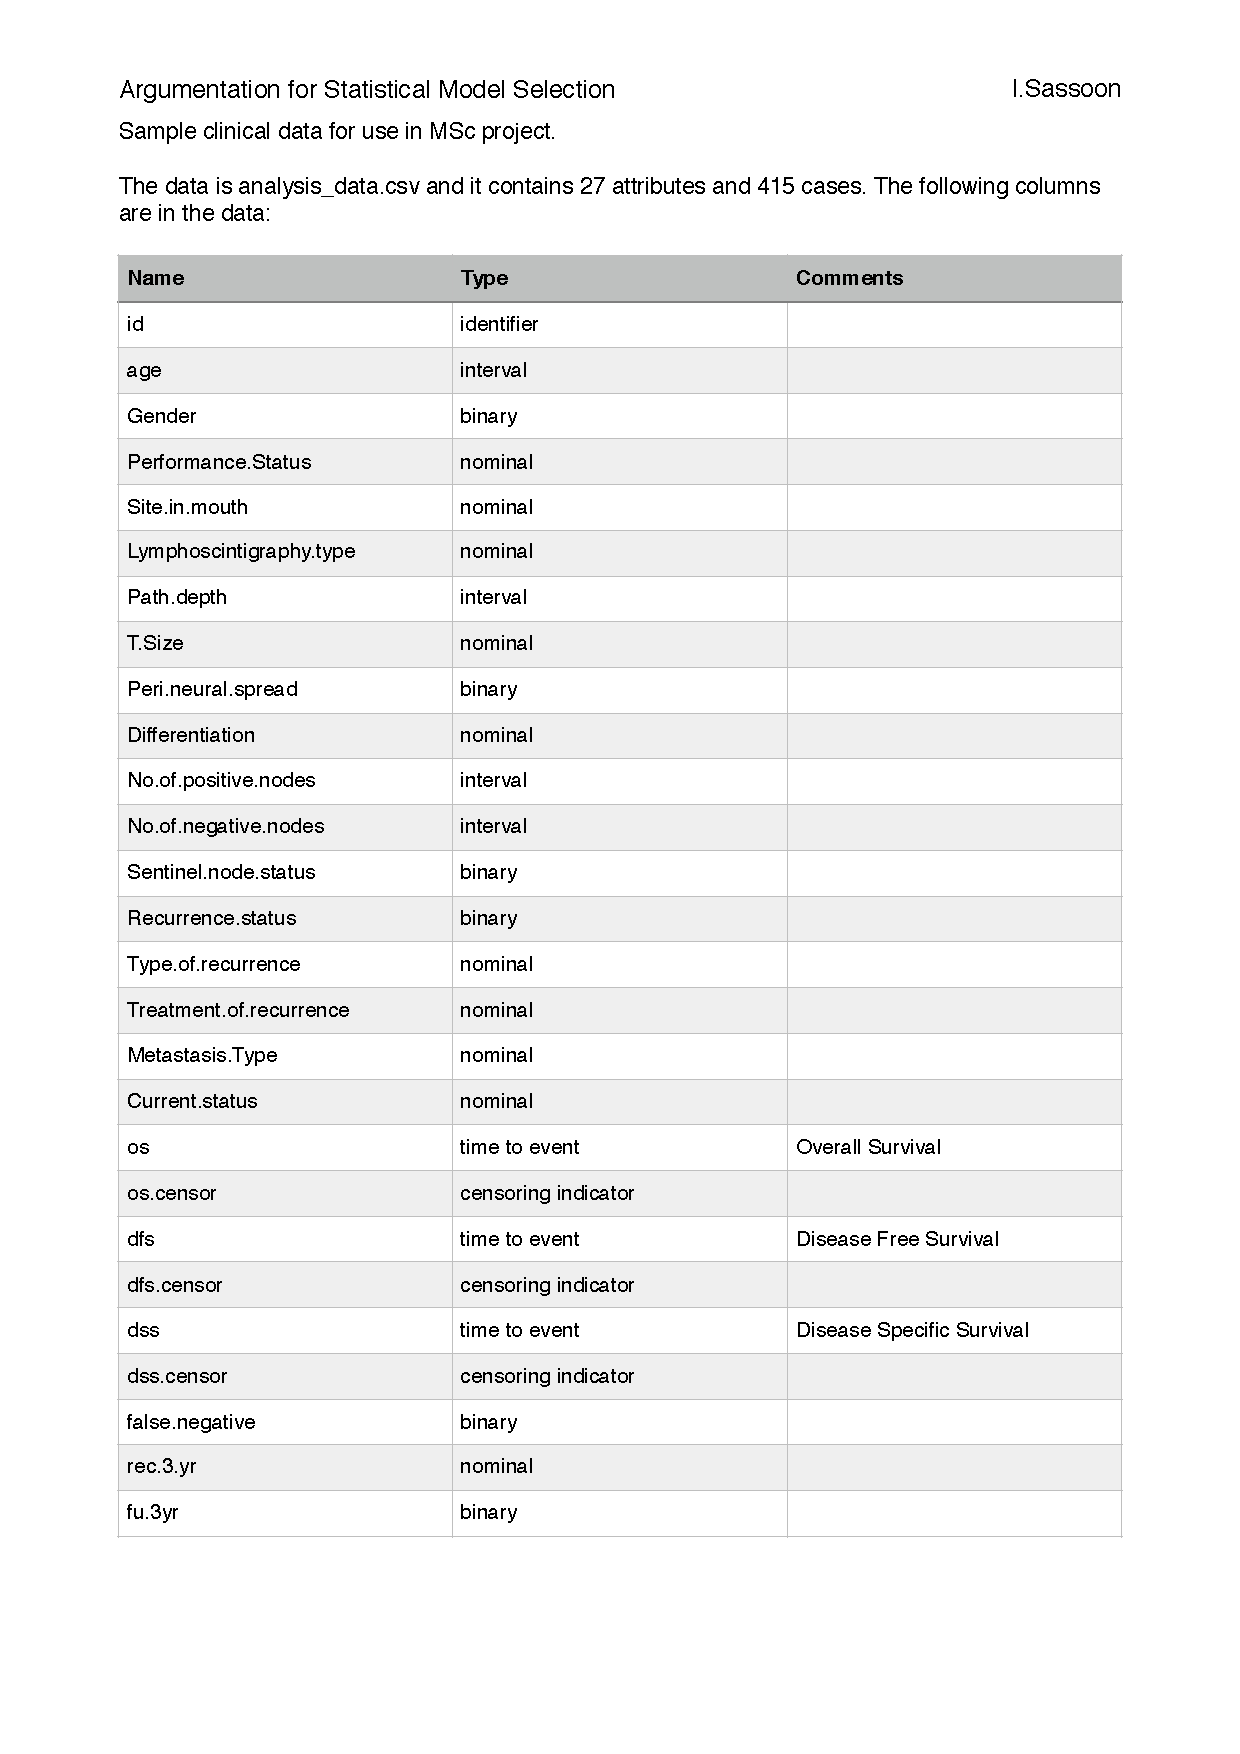
\includegraphics[page=1,width=0.85\textwidth]{appendix/analysis_data.pdf}
	\captionof{figure}{
	Explanation of the example data set provided by I. Sassoon.
	\label{fig:dataset}
	}

	\includegraphics[page=2,width=0.85\textwidth]{appendix/analysis_data.pdf}
	\captionof{figure}{Possible research questions arising from the example data set.
		\label{fig:dataset:rq}
	}
}



\section{Software related Appendix}
\label{app:b}
\subsection{Code Samples}

\begin{listing}[H]
	\centering
	\rubycode[fontsize=\tiny]{figures/eaf_to_af.rb}	
	\caption{Ruby Code to implement \autoref{fig:eaf_algo}.}
	\label{lst:eaf}
\end{listing}

\begin{listing}[H]
	\centering
	\rubycode{figures/find_pref.rb}	
	\caption{Ruby Code to implement the labelling based approach $FIND\_PREF$ presented in \autoref{fig:af_algo}.}
	\label{lst:af}
\end{listing}

\begin{listing}[hbtp]
	\rcode{figures/weibull_test.r}
	\caption{R-script to perform a \texttt{QueryTestAssumption} on a data set to check whether the Weibull-Model is applicable or not. The script generates a plot that will be stored in \texttt{fileName} and presented to the end-user.}
	\label{lst:rcode}
\end{listing}


\subsection{Installation Guide}
\label{app:installation}
The following installation guide has been tested on a clean debian OS:

\begin{enumerate}
\def\labelenumi{\arabic{enumi}.}
\item
  Install \texttt{postgresql} and \texttt{R} with:
  \texttt{sudo\ apt-get\ install\ postgresql\ r-base}
\item
  Install \texttt{rvm} following \href{https://rvm.io/rvm/install}{this
  guide}.
\item
  Clone the repository:\\
  \texttt{git\ clone\ }\url{https://github.com/sebastianzillessen/small-data-analyst.git}
\item
  \texttt{cd\ small-data-analyst}
\item
  Install the required ruby version as prompted by rvm:
  \texttt{rvm\ install\ ruby-2.2.4}
\item
  Install bundler: \texttt{gem\ install\ bundler\ foreman}
\item
  Install all required gems: \texttt{bundle\ install}
\item
  Set the AWS credentials in the file \texttt{.env}:

\begin{verbatim}
PORT=3000
AWS_ACCESS_KEY_ID=XXXXXXXXXXXXX
AWS_SECRET_ACCESS_KEY=YYYYYYYYYYYYYYYYYYYY
S3_BUCKET_NAME=ZZZZZZZZZZZZZZ
\end{verbatim}
\item Set the database credentials if required in \texttt{config/database.yml}.
\item
  Initialise the database:\\
  \texttt{rake\ db:create\ \&\&\ rake\ db:setup\ \&\&\ rake\ db:migrate}
\item
  Start the server with \texttt{foreman\ start}
\item
  Create an Admin user:

\begin{verbatim}
$ rails console
> u = User.create(email: "test1@test.de", password: "fooPassword", 
		approved: true, role: :admin)
> u.confirm!
\end{verbatim}
\item
  Navigate to \texttt{http://localhost:3000} and play around with the
  application.
\end{enumerate}


\subsection{Use Cases}
\label{app:use_cases}

Figures \ref{fig:usecase:clinician}, \ref{fig:usecase:statistician} and \ref{fig:usecase:admin} provide an overview over the implemented \glspl{use_case} in the application grouped by their main actors. A complete list of all \glspl{use_case} can be found for further references under \href{https://trello.com/b/ywCkicpc/msc-small-data-analyst}{https://trello.com/b/ywCkicpc/msc-small-data-analyst}.

% use_cases
{
	\centering
	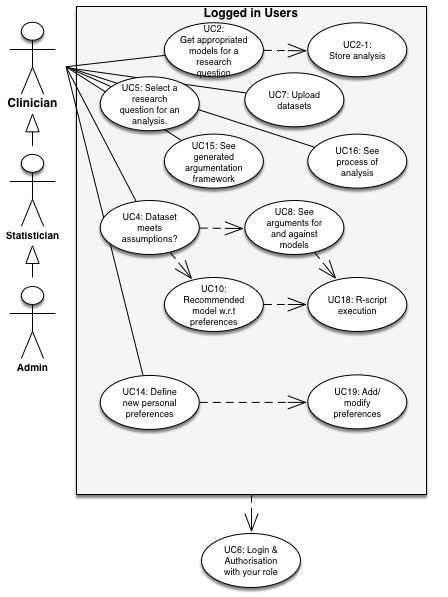
\includegraphics[width=0.6\textwidth]{figures/use_case_clinician}
	\captionof{figure}{Use Case overview for clinicians. \label{fig:usecase:clinician}}
	
	
	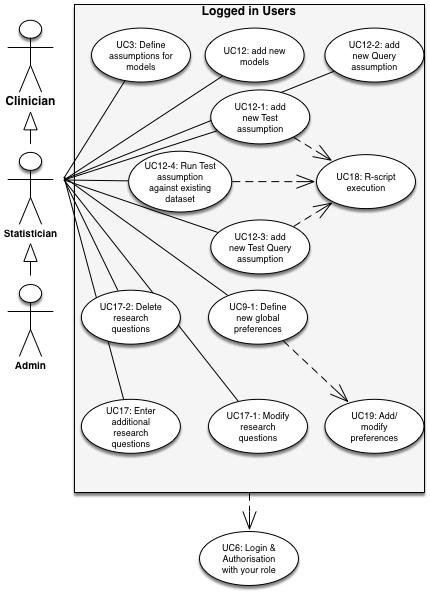
\includegraphics[width=0.6\textwidth]{figures/use_case_statistician}
	\captionof{figure}{Use Case overview for statisticians. \label{fig:usecase:statistician}}
	
	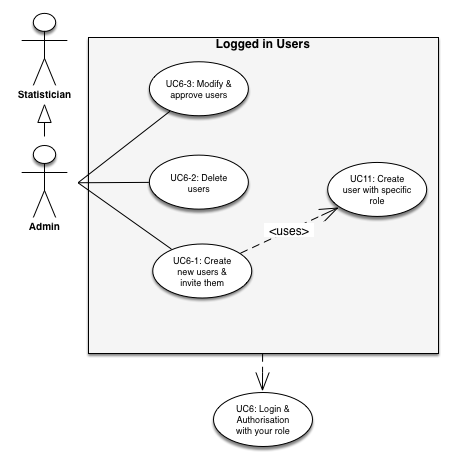
\includegraphics[width=0.6\textwidth]{figures/use_case_admin}
	\captionof{figure}{Use Case overview for administrators. \label{fig:usecase:admin}}

}

\section{Third Party Libraries}
\label{app:c}
\label{app:3rdparty}
\autoref{tab:libs} contains all the third party libraries that have been used in the project. These are all public available and free of use. Additional information can be found for each listed \texttt{gem} under \href{http://rubygems.org}{http://rubygems.org}.

\begin{table}[!h]
	\centering
	\begin{tabular}{|p{2.4cm}r||p{2.4cm}r||p{2.4cm}r|}
	\hline
	\textbf{Library} & \textbf{ver.} & 	\textbf{Library} & \textbf{ver.} & 	\textbf{Library} & \textbf{ver.} \\
	actionmailer&(4.2.6)&faker&(1.6.3)&rails\_12factor&(0.0.3)\\
actionpack&(4.2.6)&foreman&(0.82.0)&\tiny{rails\_serve\_static\_assets}&(0.0.5)\\
actionview&(4.2.6)&formtastic&(3.1.4)&\tiny{rails\_stdout\_logging}&(0.0.5)\\
activejob&(4.2.6)&\tiny{formtastic-bootstrap}&(3.1.1)&railties&(4.2.6)\\
activemodel&(4.2.6)&globalid&(0.3.6)&rake&(11.2.2)\\
activerecord&(4.2.6)&haml&(4.0.7)&rdoc&(4.2.2)\\
activesupport&(4.2.6)&haml-rails&(0.9.0)&ref&(2.0.0)\\
addressable&(2.4.0)&heroku-api&(0.4.2)&responders&(2.2.0)\\
arel&(6.0.3)&html2haml&(2.0.0)&\tiny{rootapp-rinruby}&(3.1.2)\footnote{https://github.com/sebastianzillessen/rinruby}\\
aws-sdk&(2.4.2)&i18n&(0.7.0)&rspec-core&(3.4.4)\\
aws-sdk-core&(2.4.2)&jbuilder&(2.5.0)&\tiny{rspec-expectations}&(3.4.0)\\
\tiny{aws-sdk-resources}&(2.4.2)&jmespath&(1.3.1)&rspec-mocks&(3.4.1)\\
bcrypt&(3.1.11)&jquery-rails&(4.1.1)&rspec-rails&(3.4.2)\\
\tiny{binding\_of\_caller}&(0.7.2)&\tiny{jquery-turbolinks}&(2.1.0)&rspec-retry&(0.4.5)\\
builder&(3.2.2)&jquery-ui-rails&(5.0.5)&rspec-support&(3.4.1)\\
bullet&(5.1.1)&json&(1.8.3)&ruby-graphviz&(1.2.2)\\
bundler&(1.12.5)&launchy&(2.4.3)&ruby\_parser&(3.8.2)\\
byebug&(9.0.5)&less&(2.6.0)&rush&(0.6.8)\\
cancancan&(1.15.0)&less-rails&(2.7.1)&sass&(3.4.22)\\
capybara&(2.7.1)&libv8&(3.16.*)&sass-rails&(5.0.4)\\
\tiny{capybara-screenshot}&(1.0.13)&loofah&(2.0.3)&sdoc&(0.4.1)\\
choice&(0.2.0)&mail&(2.6.4)&session&(3.2.0)\\
cliver&(0.3.2)&method\_source&(0.8.2)&sexp\_processor&(4.7.0)\\
cocoon&(1.2.9)&\tiny{mime-types}&(3.1)&\tiny{shoulda-matchers}&(3.1.1)\\
\tiny{codeclimate-test-reporter}&(0.6.0)&\tiny{mime-types-data}&(3.2016*)&simplecov&(0.12.0)\\
coderay&(1.1.1)&mini\_portile2&(2.1.0)&\tiny{simplecov-html}&(0.10.0)\\
coffee-rails&(4.1.1)&minitest&(5.9.0)&slop&(3.6.0)\\
coffee-script&(2.4.1)&multi\_json&(1.12.1)&sprockets&(3.6.2)\\
\tiny{coffee-script-source}&(1.10.0)&nokogiri&(1.6.8)&sprockets-rails&(3.0.4)\\
commonjs&(0.2.7)&orm\_adapter&(0.5.0)&teaspoon&(1.1.5)\\
\tiny{concurrent-ruby}&(1.0.2)&pg&(0.18.4)&\tiny{teaspoon-jasmine}&(2.3.4)\\
data\_migrate&(2.1.0)&pkg-config&(1.1.7)&therubyracer&(0.12.2)\\
\tiny{database\_cleaner}&(1.5.3)&poltergeist&(1.10.0)&thor&(0.19.1)\\
debug\_inspector&(0.0.2)&pry&(0.10.3)&thread\_safe&(0.3.5)\\
delayed\_job&(4.1.2)&puma&(3.4.0)&tilt&(2.0.5)\\
\tiny{delayed\_job\_active\_record}&(4.1.1)&rack&(1.6.4)&turbolinks&(2.5.3)\\
devise&(4.1.1)&\tiny{rack-mini-profiler}&(0.10.1)&\tiny{twitter-bootstrap-rails}&(3.2.2)\\
diff-lcs&(1.2.5)&rack-test&(0.6.3)&tzinfo&(1.2.2)\\plec
docile&(1.1.5)&rails&(4.2.6)&uglifier&(3.0.0)\\
dotenv&(2.1.1)&\tiny{rails-assets-chosen}&(1.6.1)&uniform\_notifier&(1.10.0)\\
dotenv-rails&(2.1.1)&\tiny{rails-assets-jquery}&(3.0.0)&warden&(1.2.6)\\
erubis&(2.7.0)&\tiny{rails-deprecated\_sanitizer}&(1.0.3)&web-console&(2.3.0)\\
excon&(0.51.0)&\tiny{rails-dom-testing}&(1.0.7)&\tiny{websocket-driver}&(0.6.4)\\
execjs&(2.7.0)&rails-erd&(1.4.7)&\tiny{websocket-extensions}&(0.1.2)\\
factory\_girl&(4.7.0)&\tiny{rails-html-sanitizer}&(1.0.3)&workless&(1.2.3)\\
factory\_girl\_rails&(4.7.0)&&&&\\
	\hline
	\end{tabular}
	\caption{Third-party libraries and services used in the web-application.}
	\label{tab:libs}
\end{table}

\clearpage
\newpage

\section{R-Spec Test Suite}
\label{app:d}
\label{app:rspec}
\sloppy
\Cref{sub:test_suit}-\ref{sub:test_suit_6} provide an impression on the developed \texttt{rspec} tests. The whole report can be as well found on \url{https://github.com/sebastianzillessen/small-data-analyst/blob/master/report.html}. 

The test suite, which is made out of $\approx 350$ specs, results in a resonable test coverage of $\geq 85\%$ (see \url{https://codeclimate.com/github/sebastianzillessen/small-data-analyst/coverage} for in depth code climate details and coverage report).


% rspec
\begin{sidewaysfigure}[!h]
	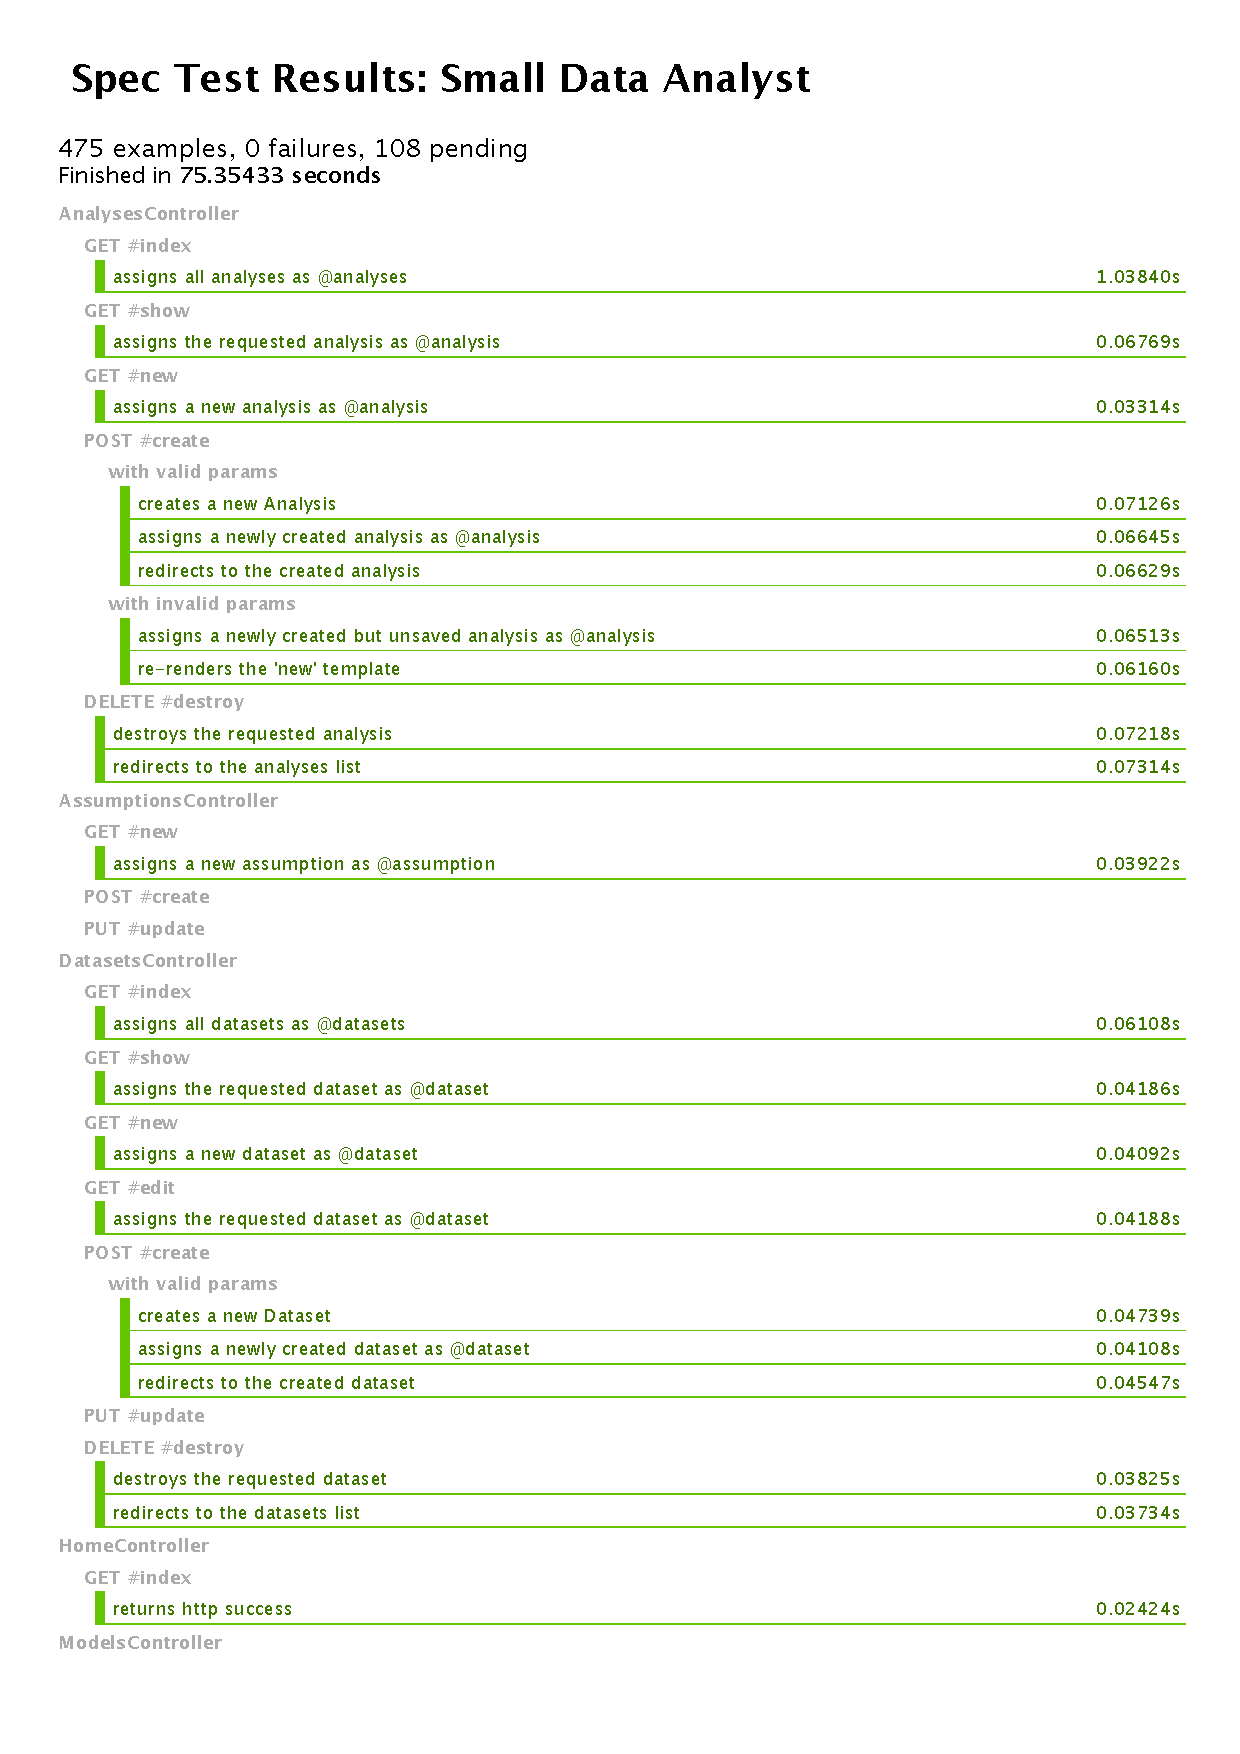
\includegraphics[page=1,width=0.5\textwidth]{appendix/RSpec}
	\includegraphics[page=2,width=0.5\textwidth]{appendix/RSpec}
	\caption{RSpec test suite export (Pages 1-2).}
	\label{sub:test_suit}
\end{sidewaysfigure}

\begin{sidewaysfigure}[!h]
	\includegraphics[page=3,width=0.5\textwidth]{appendix/RSpec}
	\includegraphics[page=4,width=0.5\textwidth]{appendix/RSpec}
	\caption{RSpec test suite export (Pages 3-4).}
	\label{sub:test_suit_2}
\end{sidewaysfigure}

\begin{sidewaysfigure}[!h]
	\includegraphics[page=5,width=0.5\textwidth]{appendix/RSpec}
	\includegraphics[page=6,width=0.5\textwidth]{appendix/RSpec}
	\caption{RSpec test suite export (Pages 5-6).}
	\label{sub:test_suit_3}
\end{sidewaysfigure}

\begin{sidewaysfigure}[!h]
	\includegraphics[page=7,width=0.5\textwidth]{appendix/RSpec}
	\includegraphics[page=8,width=0.5\textwidth]{appendix/RSpec}
	\caption{RSpec test suite export (Pages 7-8).}
	\label{sub:test_suit_4}
\end{sidewaysfigure}

\begin{sidewaysfigure}[!h]
	\includegraphics[page=9,width=0.5\textwidth]{appendix/RSpec}
	\includegraphics[page=10,width=0.5\textwidth]{appendix/RSpec}
	\caption{RSpec test suite export (Pages 9-10).}
	\label{sub:test_suit_5}
\end{sidewaysfigure}

\begin{sidewaysfigure}[!h]
	\includegraphics[page=11,width=0.5\textwidth]{appendix/RSpec}
	\includegraphics[page=12,width=0.5\textwidth]{appendix/RSpec}
	\caption{RSpec test suite export (Pages 11-12).}
	\label{sub:test_suit_6}
\end{sidewaysfigure}

\newpage
\cleardoublepage

\section{Source Code}

The core source code (without any configuration files and without any additional required scripts) of this project contains around 5000 lines of code, spread over $\approx 200$ files. Representing this in an PDF will not really help the reader to understand the project structure and its files. Hence, these files have not been included into the project. However, the source code is available on \url{https://github.com/sebastianzillessen/small-data-analyst/tree/Release} and has been tagged with "Release". This tag will not be changed anymore after the submission of the thesis. The uniq SHA1 identifier for the last commit is "\#ae5e3fff2cb1cf3ad7b23afdb39e7ea432cce69c".
%\begin{listing}[H]
      \centering
      \inputminted[fontfamily=tt,linenos=true,numbersep=5pt,gobble=0,framerule=0.4pt,framesep=2mm,funcnamehighlighting=true,tabsize=2,obeytabs=false,mathescape=falsesamepage=false, showspaces=false,showtabs =false,texcl=false,stepnumber=5,breaklines=true,fontsize=	iny]{extension}{../small_data_analyst/app/assets/javascripts/application.js}
      \caption{assets: Application (app/assets/javascripts/application.js)}
    \end{listing}
    \begin{listing}[H]
      \centering
      \inputminted[fontfamily=tt,linenos=true,numbersep=5pt,gobble=0,framerule=0.4pt,framesep=2mm,funcnamehighlighting=true,tabsize=2,obeytabs=false,mathescape=falsesamepage=false, showspaces=false,showtabs =false,texcl=false,stepnumber=5,breaklines=true,fontsize=	iny]{extension}{../small_data_analyst/app/assets/javascripts/bootstrap.js.coffee}
      \caption{assets: Bootstrap (app/assets/javascripts/bootstrap.js.coffee)}
    \end{listing}
    \begin{listing}[H]
      \centering
      \inputminted[fontfamily=tt,linenos=true,numbersep=5pt,gobble=0,framerule=0.4pt,framesep=2mm,funcnamehighlighting=true,tabsize=2,obeytabs=false,mathescape=falsesamepage=false, showspaces=false,showtabs =false,texcl=false,stepnumber=5,breaklines=true,fontsize=	iny]{extension}{../small_data_analyst/app/assets/javascripts/chosen-init.js}
      \caption{assets: Chosen-init (app/assets/javascripts/chosen-init.js)}
    \end{listing}
    \begin{listing}[H]
      \centering
      \inputminted[fontfamily=tt,linenos=true,numbersep=5pt,gobble=0,framerule=0.4pt,framesep=2mm,funcnamehighlighting=true,tabsize=2,obeytabs=false,mathescape=falsesamepage=false, showspaces=false,showtabs =false,texcl=false,stepnumber=5,breaklines=true,fontsize=	iny]{extension}{../small_data_analyst/app/assets/javascripts/click_row.js}
      \caption{assets: ClickRow (app/assets/javascripts/click\_row.js)}
    \end{listing}
    \begin{listing}[H]
      \centering
      \inputminted[fontfamily=tt,linenos=true,numbersep=5pt,gobble=0,framerule=0.4pt,framesep=2mm,funcnamehighlighting=true,tabsize=2,obeytabs=false,mathescape=falsesamepage=false, showspaces=false,showtabs =false,texcl=false,stepnumber=5,breaklines=true,fontsize=	iny]{extension}{../small_data_analyst/app/assets/javascripts/dismissable_alerts.js}
      \caption{assets: DismissableAlert (app/assets/javascripts/dismissable\_alerts.js)}
    \end{listing}
    \begin{listing}[H]
      \centering
      \inputminted[fontfamily=tt,linenos=true,numbersep=5pt,gobble=0,framerule=0.4pt,framesep=2mm,funcnamehighlighting=true,tabsize=2,obeytabs=false,mathescape=falsesamepage=false, showspaces=false,showtabs =false,texcl=false,stepnumber=5,breaklines=true,fontsize=	iny]{extension}{../small_data_analyst/app/assets/javascripts/enlarge-image.js}
      \caption{assets: Enlarge-image (app/assets/javascripts/enlarge-image.js)}
    \end{listing}
    \begin{listing}[H]
      \centering
      \inputminted[fontfamily=tt,linenos=true,numbersep=5pt,gobble=0,framerule=0.4pt,framesep=2mm,funcnamehighlighting=true,tabsize=2,obeytabs=false,mathescape=falsesamepage=false, showspaces=false,showtabs =false,texcl=false,stepnumber=5,breaklines=true,fontsize=	iny]{extension}{../small_data_analyst/app/assets/javascripts/fill_input_by_click.js}
      \caption{assets: FillInputByClick (app/assets/javascripts/fill\_input\_by\_click.js)}
    \end{listing}
    \begin{listing}[H]
      \centering
      \inputminted[fontfamily=tt,linenos=true,numbersep=5pt,gobble=0,framerule=0.4pt,framesep=2mm,funcnamehighlighting=true,tabsize=2,obeytabs=false,mathescape=falsesamepage=false, showspaces=false,showtabs =false,texcl=false,stepnumber=5,breaklines=true,fontsize=	iny]{extension}{../small_data_analyst/app/assets/javascripts/form_spinner.js}
      \caption{assets: FormSpinner (app/assets/javascripts/form\_spinner.js)}
    \end{listing}
    \begin{listing}[H]
      \centering
      \inputminted[fontfamily=tt,linenos=true,numbersep=5pt,gobble=0,framerule=0.4pt,framesep=2mm,funcnamehighlighting=true,tabsize=2,obeytabs=false,mathescape=falsesamepage=false, showspaces=false,showtabs =false,texcl=false,stepnumber=5,breaklines=true,fontsize=	iny]{extension}{../small_data_analyst/app/assets/javascripts/preferences.js}
      \caption{assets: Preference (app/assets/javascripts/preferences.js)}
    \end{listing}
    \begin{listing}[H]
      \centering
      \inputminted[fontfamily=tt,linenos=true,numbersep=5pt,gobble=0,framerule=0.4pt,framesep=2mm,funcnamehighlighting=true,tabsize=2,obeytabs=false,mathescape=falsesamepage=false, showspaces=false,showtabs =false,texcl=false,stepnumber=5,breaklines=true,fontsize=	iny]{extension}{../small_data_analyst/app/assets/javascripts/r_script_validator.js}
      \caption{assets: RScriptValidator (app/assets/javascripts/r\_script\_validator.js)}
    \end{listing}
    \begin{listing}[H]
      \centering
      \inputminted[fontfamily=tt,linenos=true,numbersep=5pt,gobble=0,framerule=0.4pt,framesep=2mm,funcnamehighlighting=true,tabsize=2,obeytabs=false,mathescape=falsesamepage=false, showspaces=false,showtabs =false,texcl=false,stepnumber=5,breaklines=true,fontsize=	iny]{extension}{../small_data_analyst/app/assets/stylesheets/_variables.scss}
      \caption{assets: Variable (app/assets/stylesheets/\_variables.scss)}
    \end{listing}
    \begin{listing}[H]
      \centering
      \inputminted[fontfamily=tt,linenos=true,numbersep=5pt,gobble=0,framerule=0.4pt,framesep=2mm,funcnamehighlighting=true,tabsize=2,obeytabs=false,mathescape=falsesamepage=false, showspaces=false,showtabs =false,texcl=false,stepnumber=5,breaklines=true,fontsize=	iny]{extension}{../small_data_analyst/app/assets/stylesheets/alert_overlay.scss}
      \caption{assets: AlertOverlay (app/assets/stylesheets/alert\_overlay.scss)}
    \end{listing}
    \begin{listing}[H]
      \centering
      \inputminted[fontfamily=tt,linenos=true,numbersep=5pt,gobble=0,framerule=0.4pt,framesep=2mm,funcnamehighlighting=true,tabsize=2,obeytabs=false,mathescape=falsesamepage=false, showspaces=false,showtabs =false,texcl=false,stepnumber=5,breaklines=true,fontsize=	iny]{extension}{../small_data_analyst/app/assets/stylesheets/application.css}
      \caption{assets: Application (app/assets/stylesheets/application.css)}
    \end{listing}
    \begin{listing}[H]
      \centering
      \inputminted[fontfamily=tt,linenos=true,numbersep=5pt,gobble=0,framerule=0.4pt,framesep=2mm,funcnamehighlighting=true,tabsize=2,obeytabs=false,mathescape=falsesamepage=false, showspaces=false,showtabs =false,texcl=false,stepnumber=5,breaklines=true,fontsize=	iny]{extension}{../small_data_analyst/app/assets/stylesheets/assumptions.scss}
      \caption{assets: Assumption (app/assets/stylesheets/assumptions.scss)}
    \end{listing}
    \begin{listing}[H]
      \centering
      \inputminted[fontfamily=tt,linenos=true,numbersep=5pt,gobble=0,framerule=0.4pt,framesep=2mm,funcnamehighlighting=true,tabsize=2,obeytabs=false,mathescape=falsesamepage=false, showspaces=false,showtabs =false,texcl=false,stepnumber=5,breaklines=true,fontsize=	iny]{extension}{../small_data_analyst/app/assets/stylesheets/bootstrap-switch.css}
      \caption{assets: Bootstrap-switch (app/assets/stylesheets/bootstrap-switch.css)}
    \end{listing}
    \begin{listing}[H]
      \centering
      \inputminted[fontfamily=tt,linenos=true,numbersep=5pt,gobble=0,framerule=0.4pt,framesep=2mm,funcnamehighlighting=true,tabsize=2,obeytabs=false,mathescape=falsesamepage=false, showspaces=false,showtabs =false,texcl=false,stepnumber=5,breaklines=true,fontsize=	iny]{extension}{../small_data_analyst/app/assets/stylesheets/bootstrap_and_overrides.css.less}
      \caption{assets: BootstrapAndOverride (app/assets/stylesheets/bootstrap\_and\_overrides.css.less)}
    \end{listing}
    \begin{listing}[H]
      \centering
      \inputminted[fontfamily=tt,linenos=true,numbersep=5pt,gobble=0,framerule=0.4pt,framesep=2mm,funcnamehighlighting=true,tabsize=2,obeytabs=false,mathescape=falsesamepage=false, showspaces=false,showtabs =false,texcl=false,stepnumber=5,breaklines=true,fontsize=	iny]{extension}{../small_data_analyst/app/assets/stylesheets/buttons.scss}
      \caption{assets: Button (app/assets/stylesheets/buttons.scss)}
    \end{listing}
    \begin{listing}[H]
      \centering
      \inputminted[fontfamily=tt,linenos=true,numbersep=5pt,gobble=0,framerule=0.4pt,framesep=2mm,funcnamehighlighting=true,tabsize=2,obeytabs=false,mathescape=falsesamepage=false, showspaces=false,showtabs =false,texcl=false,stepnumber=5,breaklines=true,fontsize=	iny]{extension}{../small_data_analyst/app/assets/stylesheets/collapse.scss}
      \caption{assets: Collapse (app/assets/stylesheets/collapse.scss)}
    \end{listing}
    \begin{listing}[H]
      \centering
      \inputminted[fontfamily=tt,linenos=true,numbersep=5pt,gobble=0,framerule=0.4pt,framesep=2mm,funcnamehighlighting=true,tabsize=2,obeytabs=false,mathescape=falsesamepage=false, showspaces=false,showtabs =false,texcl=false,stepnumber=5,breaklines=true,fontsize=	iny]{extension}{../small_data_analyst/app/assets/stylesheets/forms.scss}
      \caption{assets: Form (app/assets/stylesheets/forms.scss)}
    \end{listing}
    \begin{listing}[H]
      \centering
      \inputminted[fontfamily=tt,linenos=true,numbersep=5pt,gobble=0,framerule=0.4pt,framesep=2mm,funcnamehighlighting=true,tabsize=2,obeytabs=false,mathescape=falsesamepage=false, showspaces=false,showtabs =false,texcl=false,stepnumber=5,breaklines=true,fontsize=	iny]{extension}{../small_data_analyst/app/assets/stylesheets/home.scss}
      \caption{assets: Home (app/assets/stylesheets/home.scss)}
    \end{listing}
    \begin{listing}[H]
      \centering
      \inputminted[fontfamily=tt,linenos=true,numbersep=5pt,gobble=0,framerule=0.4pt,framesep=2mm,funcnamehighlighting=true,tabsize=2,obeytabs=false,mathescape=falsesamepage=false, showspaces=false,showtabs =false,texcl=false,stepnumber=5,breaklines=true,fontsize=	iny]{extension}{../small_data_analyst/app/assets/stylesheets/images.scss}
      \caption{assets: Image (app/assets/stylesheets/images.scss)}
    \end{listing}
    \begin{listing}[H]
      \centering
      \inputminted[fontfamily=tt,linenos=true,numbersep=5pt,gobble=0,framerule=0.4pt,framesep=2mm,funcnamehighlighting=true,tabsize=2,obeytabs=false,mathescape=falsesamepage=false, showspaces=false,showtabs =false,texcl=false,stepnumber=5,breaklines=true,fontsize=	iny]{extension}{../small_data_analyst/app/assets/stylesheets/lists.scss}
      \caption{assets: List (app/assets/stylesheets/lists.scss)}
    \end{listing}
    \begin{listing}[H]
      \centering
      \inputminted[fontfamily=tt,linenos=true,numbersep=5pt,gobble=0,framerule=0.4pt,framesep=2mm,funcnamehighlighting=true,tabsize=2,obeytabs=false,mathescape=falsesamepage=false, showspaces=false,showtabs =false,texcl=false,stepnumber=5,breaklines=true,fontsize=	iny]{extension}{../small_data_analyst/app/assets/stylesheets/r_script_validator.scss}
      \caption{assets: RScriptValidator (app/assets/stylesheets/r\_script\_validator.scss)}
    \end{listing}
    \begin{listing}[H]
      \centering
      \inputminted[fontfamily=tt,linenos=true,numbersep=5pt,gobble=0,framerule=0.4pt,framesep=2mm,funcnamehighlighting=true,tabsize=2,obeytabs=false,mathescape=falsesamepage=false, showspaces=false,showtabs =false,texcl=false,stepnumber=5,breaklines=true,fontsize=	iny]{extension}{../small_data_analyst/app/assets/stylesheets/scaffolds.scss}
      \caption{assets: Scaffold (app/assets/stylesheets/scaffolds.scss)}
    \end{listing}
    \begin{listing}[H]
      \centering
      \inputminted[fontfamily=tt,linenos=true,numbersep=5pt,gobble=0,framerule=0.4pt,framesep=2mm,funcnamehighlighting=true,tabsize=2,obeytabs=false,mathescape=falsesamepage=false, showspaces=false,showtabs =false,texcl=false,stepnumber=5,breaklines=true,fontsize=	iny]{extension}{../small_data_analyst/app/assets/stylesheets/sortable.scss}
      \caption{assets: Sortable (app/assets/stylesheets/sortable.scss)}
    \end{listing}
    \begin{listing}[H]
      \centering
      \inputminted[fontfamily=tt,linenos=true,numbersep=5pt,gobble=0,framerule=0.4pt,framesep=2mm,funcnamehighlighting=true,tabsize=2,obeytabs=false,mathescape=falsesamepage=false, showspaces=false,showtabs =false,texcl=false,stepnumber=5,breaklines=true,fontsize=	iny]{extension}{../small_data_analyst/app/assets/stylesheets/tables.scss}
      \caption{assets: Table (app/assets/stylesheets/tables.scss)}
    \end{listing}
    \begin{listing}[H]
      \centering
      \inputminted[fontfamily=tt,linenos=true,numbersep=5pt,gobble=0,framerule=0.4pt,framesep=2mm,funcnamehighlighting=true,tabsize=2,obeytabs=false,mathescape=falsesamepage=false, showspaces=false,showtabs =false,texcl=false,stepnumber=5,breaklines=true,fontsize=	iny]{extension}{../small_data_analyst/app/controllers/admin/admin_controller.rb}
      \caption{controllers: AdminController (app/controllers/admin/admin\_controller.rb)}
    \end{listing}
    \begin{listing}[H]
      \centering
      \inputminted[fontfamily=tt,linenos=true,numbersep=5pt,gobble=0,framerule=0.4pt,framesep=2mm,funcnamehighlighting=true,tabsize=2,obeytabs=false,mathescape=falsesamepage=false, showspaces=false,showtabs =false,texcl=false,stepnumber=5,breaklines=true,fontsize=	iny]{extension}{../small_data_analyst/app/controllers/admin/users_controller.rb}
      \caption{controllers: UsersController (app/controllers/admin/users\_controller.rb)}
    \end{listing}
    \begin{listing}[H]
      \centering
      \inputminted[fontfamily=tt,linenos=true,numbersep=5pt,gobble=0,framerule=0.4pt,framesep=2mm,funcnamehighlighting=true,tabsize=2,obeytabs=false,mathescape=falsesamepage=false, showspaces=false,showtabs =false,texcl=false,stepnumber=5,breaklines=true,fontsize=	iny]{extension}{../small_data_analyst/app/controllers/analyses_controller.rb}
      \caption{controllers: AnalysesController (app/controllers/analyses\_controller.rb)}
    \end{listing}
    \begin{listing}[H]
      \centering
      \inputminted[fontfamily=tt,linenos=true,numbersep=5pt,gobble=0,framerule=0.4pt,framesep=2mm,funcnamehighlighting=true,tabsize=2,obeytabs=false,mathescape=falsesamepage=false, showspaces=false,showtabs =false,texcl=false,stepnumber=5,breaklines=true,fontsize=	iny]{extension}{../small_data_analyst/app/controllers/application_controller.rb}
      \caption{controllers: ApplicationController (app/controllers/application\_controller.rb)}
    \end{listing}
    \begin{listing}[H]
      \centering
      \inputminted[fontfamily=tt,linenos=true,numbersep=5pt,gobble=0,framerule=0.4pt,framesep=2mm,funcnamehighlighting=true,tabsize=2,obeytabs=false,mathescape=falsesamepage=false, showspaces=false,showtabs =false,texcl=false,stepnumber=5,breaklines=true,fontsize=	iny]{extension}{../small_data_analyst/app/controllers/assumptions_controller.rb}
      \caption{controllers: AssumptionsController (app/controllers/assumptions\_controller.rb)}
    \end{listing}
    \begin{listing}[H]
      \centering
      \inputminted[fontfamily=tt,linenos=true,numbersep=5pt,gobble=0,framerule=0.4pt,framesep=2mm,funcnamehighlighting=true,tabsize=2,obeytabs=false,mathescape=falsesamepage=false, showspaces=false,showtabs =false,texcl=false,stepnumber=5,breaklines=true,fontsize=	iny]{extension}{../small_data_analyst/app/controllers/confirmations_controller.rb}
      \caption{controllers: ConfirmationsController (app/controllers/confirmations\_controller.rb)}
    \end{listing}
    \begin{listing}[H]
      \centering
      \inputminted[fontfamily=tt,linenos=true,numbersep=5pt,gobble=0,framerule=0.4pt,framesep=2mm,funcnamehighlighting=true,tabsize=2,obeytabs=false,mathescape=falsesamepage=false, showspaces=false,showtabs =false,texcl=false,stepnumber=5,breaklines=true,fontsize=	iny]{extension}{../small_data_analyst/app/controllers/datasets_controller.rb}
      \caption{controllers: DatasetsController (app/controllers/datasets\_controller.rb)}
    \end{listing}
    \begin{listing}[H]
      \centering
      \inputminted[fontfamily=tt,linenos=true,numbersep=5pt,gobble=0,framerule=0.4pt,framesep=2mm,funcnamehighlighting=true,tabsize=2,obeytabs=false,mathescape=falsesamepage=false, showspaces=false,showtabs =false,texcl=false,stepnumber=5,breaklines=true,fontsize=	iny]{extension}{../small_data_analyst/app/controllers/home_controller.rb}
      \caption{controllers: HomeController (app/controllers/home\_controller.rb)}
    \end{listing}
    \begin{listing}[H]
      \centering
      \inputminted[fontfamily=tt,linenos=true,numbersep=5pt,gobble=0,framerule=0.4pt,framesep=2mm,funcnamehighlighting=true,tabsize=2,obeytabs=false,mathescape=falsesamepage=false, showspaces=false,showtabs =false,texcl=false,stepnumber=5,breaklines=true,fontsize=	iny]{extension}{../small_data_analyst/app/controllers/models_controller.rb}
      \caption{controllers: ModelsController (app/controllers/models\_controller.rb)}
    \end{listing}
    \begin{listing}[H]
      \centering
      \inputminted[fontfamily=tt,linenos=true,numbersep=5pt,gobble=0,framerule=0.4pt,framesep=2mm,funcnamehighlighting=true,tabsize=2,obeytabs=false,mathescape=falsesamepage=false, showspaces=false,showtabs =false,texcl=false,stepnumber=5,breaklines=true,fontsize=	iny]{extension}{../small_data_analyst/app/controllers/preferences_controller.rb}
      \caption{controllers: PreferencesController (app/controllers/preferences\_controller.rb)}
    \end{listing}
    \begin{listing}[H]
      \centering
      \inputminted[fontfamily=tt,linenos=true,numbersep=5pt,gobble=0,framerule=0.4pt,framesep=2mm,funcnamehighlighting=true,tabsize=2,obeytabs=false,mathescape=falsesamepage=false, showspaces=false,showtabs =false,texcl=false,stepnumber=5,breaklines=true,fontsize=	iny]{extension}{../small_data_analyst/app/controllers/query_assumption_results_controller.rb}
      \caption{controllers: QueryAssumptionResultsController (app/controllers/query\_assumption\_results\_controller.rb)}
    \end{listing}
    \begin{listing}[H]
      \centering
      \inputminted[fontfamily=tt,linenos=true,numbersep=5pt,gobble=0,framerule=0.4pt,framesep=2mm,funcnamehighlighting=true,tabsize=2,obeytabs=false,mathescape=falsesamepage=false, showspaces=false,showtabs =false,texcl=false,stepnumber=5,breaklines=true,fontsize=	iny]{extension}{../small_data_analyst/app/controllers/r_scripts_controller.rb}
      \caption{controllers: RScriptsController (app/controllers/r\_scripts\_controller.rb)}
    \end{listing}
    \begin{listing}[H]
      \centering
      \inputminted[fontfamily=tt,linenos=true,numbersep=5pt,gobble=0,framerule=0.4pt,framesep=2mm,funcnamehighlighting=true,tabsize=2,obeytabs=false,mathescape=falsesamepage=false, showspaces=false,showtabs =false,texcl=false,stepnumber=5,breaklines=true,fontsize=	iny]{extension}{../small_data_analyst/app/controllers/research_questions_controller.rb}
      \caption{controllers: ResearchQuestionsController (app/controllers/research\_questions\_controller.rb)}
    \end{listing}
    \begin{listing}[H]
      \centering
      \inputminted[fontfamily=tt,linenos=true,numbersep=5pt,gobble=0,framerule=0.4pt,framesep=2mm,funcnamehighlighting=true,tabsize=2,obeytabs=false,mathescape=falsesamepage=false, showspaces=false,showtabs =false,texcl=false,stepnumber=5,breaklines=true,fontsize=	iny]{extension}{../small_data_analyst/app/helpers/analyses_helper.rb}
      \caption{helpers: AnalysesHelper (app/helpers/analyses\_helper.rb)}
    \end{listing}
    \begin{listing}[H]
      \centering
      \inputminted[fontfamily=tt,linenos=true,numbersep=5pt,gobble=0,framerule=0.4pt,framesep=2mm,funcnamehighlighting=true,tabsize=2,obeytabs=false,mathescape=falsesamepage=false, showspaces=false,showtabs =false,texcl=false,stepnumber=5,breaklines=true,fontsize=	iny]{extension}{../small_data_analyst/app/helpers/application_helper.rb}
      \caption{helpers: ApplicationHelper (app/helpers/application\_helper.rb)}
    \end{listing}
    \begin{listing}[H]
      \centering
      \inputminted[fontfamily=tt,linenos=true,numbersep=5pt,gobble=0,framerule=0.4pt,framesep=2mm,funcnamehighlighting=true,tabsize=2,obeytabs=false,mathescape=falsesamepage=false, showspaces=false,showtabs =false,texcl=false,stepnumber=5,breaklines=true,fontsize=	iny]{extension}{../small_data_analyst/app/helpers/assumptions_helper.rb}
      \caption{helpers: AssumptionsHelper (app/helpers/assumptions\_helper.rb)}
    \end{listing}
    \begin{listing}[H]
      \centering
      \inputminted[fontfamily=tt,linenos=true,numbersep=5pt,gobble=0,framerule=0.4pt,framesep=2mm,funcnamehighlighting=true,tabsize=2,obeytabs=false,mathescape=falsesamepage=false, showspaces=false,showtabs =false,texcl=false,stepnumber=5,breaklines=true,fontsize=	iny]{extension}{../small_data_analyst/app/helpers/button_helper.rb}
      \caption{helpers: ButtonHelper (app/helpers/button\_helper.rb)}
    \end{listing}
    \begin{listing}[H]
      \centering
      \inputminted[fontfamily=tt,linenos=true,numbersep=5pt,gobble=0,framerule=0.4pt,framesep=2mm,funcnamehighlighting=true,tabsize=2,obeytabs=false,mathescape=falsesamepage=false, showspaces=false,showtabs =false,texcl=false,stepnumber=5,breaklines=true,fontsize=	iny]{extension}{../small_data_analyst/app/helpers/datasets_helper.rb}
      \caption{helpers: DatasetsHelper (app/helpers/datasets\_helper.rb)}
    \end{listing}
    \begin{listing}[H]
      \centering
      \inputminted[fontfamily=tt,linenos=true,numbersep=5pt,gobble=0,framerule=0.4pt,framesep=2mm,funcnamehighlighting=true,tabsize=2,obeytabs=false,mathescape=falsesamepage=false, showspaces=false,showtabs =false,texcl=false,stepnumber=5,breaklines=true,fontsize=	iny]{extension}{../small_data_analyst/app/helpers/devise_helper.rb}
      \caption{helpers: DeviseHelper (app/helpers/devise\_helper.rb)}
    \end{listing}
    \begin{listing}[H]
      \centering
      \inputminted[fontfamily=tt,linenos=true,numbersep=5pt,gobble=0,framerule=0.4pt,framesep=2mm,funcnamehighlighting=true,tabsize=2,obeytabs=false,mathescape=falsesamepage=false, showspaces=false,showtabs =false,texcl=false,stepnumber=5,breaklines=true,fontsize=	iny]{extension}{../small_data_analyst/app/helpers/home_helper.rb}
      \caption{helpers: HomeHelper (app/helpers/home\_helper.rb)}
    \end{listing}
    \begin{listing}[H]
      \centering
      \inputminted[fontfamily=tt,linenos=true,numbersep=5pt,gobble=0,framerule=0.4pt,framesep=2mm,funcnamehighlighting=true,tabsize=2,obeytabs=false,mathescape=falsesamepage=false, showspaces=false,showtabs =false,texcl=false,stepnumber=5,breaklines=true,fontsize=	iny]{extension}{../small_data_analyst/app/helpers/models_helper.rb}
      \caption{helpers: ModelsHelper (app/helpers/models\_helper.rb)}
    \end{listing}
    \begin{listing}[H]
      \centering
      \inputminted[fontfamily=tt,linenos=true,numbersep=5pt,gobble=0,framerule=0.4pt,framesep=2mm,funcnamehighlighting=true,tabsize=2,obeytabs=false,mathescape=falsesamepage=false, showspaces=false,showtabs =false,texcl=false,stepnumber=5,breaklines=true,fontsize=	iny]{extension}{../small_data_analyst/app/helpers/preferences_helper.rb}
      \caption{helpers: PreferencesHelper (app/helpers/preferences\_helper.rb)}
    \end{listing}
    \begin{listing}[H]
      \centering
      \inputminted[fontfamily=tt,linenos=true,numbersep=5pt,gobble=0,framerule=0.4pt,framesep=2mm,funcnamehighlighting=true,tabsize=2,obeytabs=false,mathescape=falsesamepage=false, showspaces=false,showtabs =false,texcl=false,stepnumber=5,breaklines=true,fontsize=	iny]{extension}{../small_data_analyst/app/helpers/query_assumption_results_helper.rb}
      \caption{helpers: QueryAssumptionResultsHelper (app/helpers/query\_assumption\_results\_helper.rb)}
    \end{listing}
    \begin{listing}[H]
      \centering
      \inputminted[fontfamily=tt,linenos=true,numbersep=5pt,gobble=0,framerule=0.4pt,framesep=2mm,funcnamehighlighting=true,tabsize=2,obeytabs=false,mathescape=falsesamepage=false, showspaces=false,showtabs =false,texcl=false,stepnumber=5,breaklines=true,fontsize=	iny]{extension}{../small_data_analyst/app/helpers/r_script_validator_helper.rb}
      \caption{helpers: RScriptValidatorHelper (app/helpers/r\_script\_validator\_helper.rb)}
    \end{listing}
    \begin{listing}[H]
      \centering
      \inputminted[fontfamily=tt,linenos=true,numbersep=5pt,gobble=0,framerule=0.4pt,framesep=2mm,funcnamehighlighting=true,tabsize=2,obeytabs=false,mathescape=falsesamepage=false, showspaces=false,showtabs =false,texcl=false,stepnumber=5,breaklines=true,fontsize=	iny]{extension}{../small_data_analyst/app/helpers/research_questions_helper.rb}
      \caption{helpers: ResearchQuestionsHelper (app/helpers/research\_questions\_helper.rb)}
    \end{listing}
    \begin{listing}[H]
      \centering
      \inputminted[fontfamily=tt,linenos=true,numbersep=5pt,gobble=0,framerule=0.4pt,framesep=2mm,funcnamehighlighting=true,tabsize=2,obeytabs=false,mathescape=falsesamepage=false, showspaces=false,showtabs =false,texcl=false,stepnumber=5,breaklines=true,fontsize=	iny]{extension}{../small_data_analyst/app/helpers/table_helper.rb}
      \caption{helpers: TableHelper (app/helpers/table\_helper.rb)}
    \end{listing}
    \begin{listing}[H]
      \centering
      \inputminted[fontfamily=tt,linenos=true,numbersep=5pt,gobble=0,framerule=0.4pt,framesep=2mm,funcnamehighlighting=true,tabsize=2,obeytabs=false,mathescape=falsesamepage=false, showspaces=false,showtabs =false,texcl=false,stepnumber=5,breaklines=true,fontsize=	iny]{extension}{../small_data_analyst/app/helpers/users_helper.rb}
      \caption{helpers: UsersHelper (app/helpers/users\_helper.rb)}
    \end{listing}
    \begin{listing}[H]
      \centering
      \inputminted[fontfamily=tt,linenos=true,numbersep=5pt,gobble=0,framerule=0.4pt,framesep=2mm,funcnamehighlighting=true,tabsize=2,obeytabs=false,mathescape=falsesamepage=false, showspaces=false,showtabs =false,texcl=false,stepnumber=5,breaklines=true,fontsize=	iny]{extension}{../small_data_analyst/app/jobs/file_deleter_job.rb}
      \caption{jobs: FileDeleterJob (app/jobs/file\_deleter\_job.rb)}
    \end{listing}
    \begin{listing}[H]
      \centering
      \inputminted[fontfamily=tt,linenos=true,numbersep=5pt,gobble=0,framerule=0.4pt,framesep=2mm,funcnamehighlighting=true,tabsize=2,obeytabs=false,mathescape=falsesamepage=false, showspaces=false,showtabs =false,texcl=false,stepnumber=5,breaklines=true,fontsize=	iny]{extension}{../small_data_analyst/app/mailers/admin_mailer.rb}
      \caption{mailers: AdminMailer (app/mailers/admin\_mailer.rb)}
    \end{listing}
    \begin{listing}[H]
      \centering
      \inputminted[fontfamily=tt,linenos=true,numbersep=5pt,gobble=0,framerule=0.4pt,framesep=2mm,funcnamehighlighting=true,tabsize=2,obeytabs=false,mathescape=falsesamepage=false, showspaces=false,showtabs =false,texcl=false,stepnumber=5,breaklines=true,fontsize=	iny]{extension}{../small_data_analyst/app/mailers/application_mailer.rb}
      \caption{mailers: ApplicationMailer (app/mailers/application\_mailer.rb)}
    \end{listing}
    \begin{listing}[H]
      \centering
      \inputminted[fontfamily=tt,linenos=true,numbersep=5pt,gobble=0,framerule=0.4pt,framesep=2mm,funcnamehighlighting=true,tabsize=2,obeytabs=false,mathescape=falsesamepage=false, showspaces=false,showtabs =false,texcl=false,stepnumber=5,breaklines=true,fontsize=	iny]{extension}{../small_data_analyst/app/models/ability.rb}
      \caption{models: Ability (app/models/ability.rb)}
    \end{listing}
    \begin{listing}[H]
      \centering
      \inputminted[fontfamily=tt,linenos=true,numbersep=5pt,gobble=0,framerule=0.4pt,framesep=2mm,funcnamehighlighting=true,tabsize=2,obeytabs=false,mathescape=falsesamepage=false, showspaces=false,showtabs =false,texcl=false,stepnumber=5,breaklines=true,fontsize=	iny]{extension}{../small_data_analyst/app/models/admin/user.rb}
      \caption{models: User (app/models/admin/user.rb)}
    \end{listing}
    \begin{listing}[H]
      \centering
      \inputminted[fontfamily=tt,linenos=true,numbersep=5pt,gobble=0,framerule=0.4pt,framesep=2mm,funcnamehighlighting=true,tabsize=2,obeytabs=false,mathescape=falsesamepage=false, showspaces=false,showtabs =false,texcl=false,stepnumber=5,breaklines=true,fontsize=	iny]{extension}{../small_data_analyst/app/models/analysis.rb}
      \caption{models: Analysis (app/models/analysis.rb)}
    \end{listing}
    \begin{listing}[H]
      \centering
      \inputminted[fontfamily=tt,linenos=true,numbersep=5pt,gobble=0,framerule=0.4pt,framesep=2mm,funcnamehighlighting=true,tabsize=2,obeytabs=false,mathescape=falsesamepage=false, showspaces=false,showtabs =false,texcl=false,stepnumber=5,breaklines=true,fontsize=	iny]{extension}{../small_data_analyst/app/models/assumption.rb}
      \caption{models: Assumption (app/models/assumption.rb)}
    \end{listing}
    \begin{listing}[H]
      \centering
      \inputminted[fontfamily=tt,linenos=true,numbersep=5pt,gobble=0,framerule=0.4pt,framesep=2mm,funcnamehighlighting=true,tabsize=2,obeytabs=false,mathescape=falsesamepage=false, showspaces=false,showtabs =false,texcl=false,stepnumber=5,breaklines=true,fontsize=	iny]{extension}{../small_data_analyst/app/models/assumptions/blank_assumption.rb}
      \caption{models: BlankAssumption (app/models/assumptions/blank\_assumption.rb)}
    \end{listing}
    \begin{listing}[H]
      \centering
      \inputminted[fontfamily=tt,linenos=true,numbersep=5pt,gobble=0,framerule=0.4pt,framesep=2mm,funcnamehighlighting=true,tabsize=2,obeytabs=false,mathescape=falsesamepage=false, showspaces=false,showtabs =false,texcl=false,stepnumber=5,breaklines=true,fontsize=	iny]{extension}{../small_data_analyst/app/models/assumptions/query_assumption.rb}
      \caption{models: QueryAssumption (app/models/assumptions/query\_assumption.rb)}
    \end{listing}
    \begin{listing}[H]
      \centering
      \inputminted[fontfamily=tt,linenos=true,numbersep=5pt,gobble=0,framerule=0.4pt,framesep=2mm,funcnamehighlighting=true,tabsize=2,obeytabs=false,mathescape=falsesamepage=false, showspaces=false,showtabs =false,texcl=false,stepnumber=5,breaklines=true,fontsize=	iny]{extension}{../small_data_analyst/app/models/assumptions/query_test_assumption.rb}
      \caption{models: QueryTestAssumption (app/models/assumptions/query\_test\_assumption.rb)}
    \end{listing}
    \begin{listing}[H]
      \centering
      \inputminted[fontfamily=tt,linenos=true,numbersep=5pt,gobble=0,framerule=0.4pt,framesep=2mm,funcnamehighlighting=true,tabsize=2,obeytabs=false,mathescape=falsesamepage=false, showspaces=false,showtabs =false,texcl=false,stepnumber=5,breaklines=true,fontsize=	iny]{extension}{../small_data_analyst/app/models/assumptions/test_assumption.rb}
      \caption{models: TestAssumption (app/models/assumptions/test\_assumption.rb)}
    \end{listing}
    \begin{listing}[H]
      \centering
      \inputminted[fontfamily=tt,linenos=true,numbersep=5pt,gobble=0,framerule=0.4pt,framesep=2mm,funcnamehighlighting=true,tabsize=2,obeytabs=false,mathescape=falsesamepage=false, showspaces=false,showtabs =false,texcl=false,stepnumber=5,breaklines=true,fontsize=	iny]{extension}{../small_data_analyst/app/models/dataset.rb}
      \caption{models: Dataset (app/models/dataset.rb)}
    \end{listing}
    \begin{listing}[H]
      \centering
      \inputminted[fontfamily=tt,linenos=true,numbersep=5pt,gobble=0,framerule=0.4pt,framesep=2mm,funcnamehighlighting=true,tabsize=2,obeytabs=false,mathescape=falsesamepage=false, showspaces=false,showtabs =false,texcl=false,stepnumber=5,breaklines=true,fontsize=	iny]{extension}{../small_data_analyst/app/models/dataset_test_assumption_result.rb}
      \caption{models: DatasetTestAssumptionResult (app/models/dataset\_test\_assumption\_result.rb)}
    \end{listing}
    \begin{listing}[H]
      \centering
      \inputminted[fontfamily=tt,linenos=true,numbersep=5pt,gobble=0,framerule=0.4pt,framesep=2mm,funcnamehighlighting=true,tabsize=2,obeytabs=false,mathescape=falsesamepage=false, showspaces=false,showtabs =false,texcl=false,stepnumber=5,breaklines=true,fontsize=	iny]{extension}{../small_data_analyst/app/models/model.rb}
      \caption{models: Model (app/models/model.rb)}
    \end{listing}
    \begin{listing}[H]
      \centering
      \inputminted[fontfamily=tt,linenos=true,numbersep=5pt,gobble=0,framerule=0.4pt,framesep=2mm,funcnamehighlighting=true,tabsize=2,obeytabs=false,mathescape=falsesamepage=false, showspaces=false,showtabs =false,texcl=false,stepnumber=5,breaklines=true,fontsize=	iny]{extension}{../small_data_analyst/app/models/model_order.rb}
      \caption{models: ModelOrder (app/models/model\_order.rb)}
    \end{listing}
    \begin{listing}[H]
      \centering
      \inputminted[fontfamily=tt,linenos=true,numbersep=5pt,gobble=0,framerule=0.4pt,framesep=2mm,funcnamehighlighting=true,tabsize=2,obeytabs=false,mathescape=falsesamepage=false, showspaces=false,showtabs =false,texcl=false,stepnumber=5,breaklines=true,fontsize=	iny]{extension}{../small_data_analyst/app/models/plot.rb}
      \caption{models: Plot (app/models/plot.rb)}
    \end{listing}
    \begin{listing}[H]
      \centering
      \inputminted[fontfamily=tt,linenos=true,numbersep=5pt,gobble=0,framerule=0.4pt,framesep=2mm,funcnamehighlighting=true,tabsize=2,obeytabs=false,mathescape=falsesamepage=false, showspaces=false,showtabs =false,texcl=false,stepnumber=5,breaklines=true,fontsize=	iny]{extension}{../small_data_analyst/app/models/possible_model.rb}
      \caption{models: PossibleModel (app/models/possible\_model.rb)}
    \end{listing}
    \begin{listing}[H]
      \centering
      \inputminted[fontfamily=tt,linenos=true,numbersep=5pt,gobble=0,framerule=0.4pt,framesep=2mm,funcnamehighlighting=true,tabsize=2,obeytabs=false,mathescape=falsesamepage=false, showspaces=false,showtabs =false,texcl=false,stepnumber=5,breaklines=true,fontsize=	iny]{extension}{../small_data_analyst/app/models/preference.rb}
      \caption{models: Preference (app/models/preference.rb)}
    \end{listing}
    \begin{listing}[H]
      \centering
      \inputminted[fontfamily=tt,linenos=true,numbersep=5pt,gobble=0,framerule=0.4pt,framesep=2mm,funcnamehighlighting=true,tabsize=2,obeytabs=false,mathescape=falsesamepage=false, showspaces=false,showtabs =false,texcl=false,stepnumber=5,breaklines=true,fontsize=	iny]{extension}{../small_data_analyst/app/models/preference_argument.rb}
      \caption{models: PreferenceArgument (app/models/preference\_argument.rb)}
    \end{listing}
    \begin{listing}[H]
      \centering
      \inputminted[fontfamily=tt,linenos=true,numbersep=5pt,gobble=0,framerule=0.4pt,framesep=2mm,funcnamehighlighting=true,tabsize=2,obeytabs=false,mathescape=falsesamepage=false, showspaces=false,showtabs =false,texcl=false,stepnumber=5,breaklines=true,fontsize=	iny]{extension}{../small_data_analyst/app/models/preference_query_assumption_result.rb}
      \caption{models: PreferenceQueryAssumptionResult (app/models/preference\_query\_assumption\_result.rb)}
    \end{listing}
    \begin{listing}[H]
      \centering
      \inputminted[fontfamily=tt,linenos=true,numbersep=5pt,gobble=0,framerule=0.4pt,framesep=2mm,funcnamehighlighting=true,tabsize=2,obeytabs=false,mathescape=falsesamepage=false, showspaces=false,showtabs =false,texcl=false,stepnumber=5,breaklines=true,fontsize=	iny]{extension}{../small_data_analyst/app/models/query_assumption_result.rb}
      \caption{models: QueryAssumptionResult (app/models/query\_assumption\_result.rb)}
    \end{listing}
    \begin{listing}[H]
      \centering
      \inputminted[fontfamily=tt,linenos=true,numbersep=5pt,gobble=0,framerule=0.4pt,framesep=2mm,funcnamehighlighting=true,tabsize=2,obeytabs=false,mathescape=falsesamepage=false, showspaces=false,showtabs =false,texcl=false,stepnumber=5,breaklines=true,fontsize=	iny]{extension}{../small_data_analyst/app/models/query_test_assumption_plot.rb}
      \caption{models: QueryTestAssumptionPlot (app/models/query\_test\_assumption\_plot.rb)}
    \end{listing}
    \begin{listing}[H]
      \centering
      \inputminted[fontfamily=tt,linenos=true,numbersep=5pt,gobble=0,framerule=0.4pt,framesep=2mm,funcnamehighlighting=true,tabsize=2,obeytabs=false,mathescape=falsesamepage=false, showspaces=false,showtabs =false,texcl=false,stepnumber=5,breaklines=true,fontsize=	iny]{extension}{../small_data_analyst/app/models/reason.rb}
      \caption{models: Reason (app/models/reason.rb)}
    \end{listing}
    \begin{listing}[H]
      \centering
      \inputminted[fontfamily=tt,linenos=true,numbersep=5pt,gobble=0,framerule=0.4pt,framesep=2mm,funcnamehighlighting=true,tabsize=2,obeytabs=false,mathescape=falsesamepage=false, showspaces=false,showtabs =false,texcl=false,stepnumber=5,breaklines=true,fontsize=	iny]{extension}{../small_data_analyst/app/models/research_question.rb}
      \caption{models: ResearchQuestion (app/models/research\_question.rb)}
    \end{listing}
    \begin{listing}[H]
      \centering
      \inputminted[fontfamily=tt,linenos=true,numbersep=5pt,gobble=0,framerule=0.4pt,framesep=2mm,funcnamehighlighting=true,tabsize=2,obeytabs=false,mathescape=falsesamepage=false, showspaces=false,showtabs =false,texcl=false,stepnumber=5,breaklines=true,fontsize=	iny]{extension}{../small_data_analyst/app/models/user.rb}
      \caption{models: User (app/models/user.rb)}
    \end{listing}
    \begin{listing}[H]
      \centering
      \inputminted[fontfamily=tt,linenos=true,numbersep=5pt,gobble=0,framerule=0.4pt,framesep=2mm,funcnamehighlighting=true,tabsize=2,obeytabs=false,mathescape=falsesamepage=false, showspaces=false,showtabs =false,texcl=false,stepnumber=5,breaklines=true,fontsize=	iny]{extension}{../small_data_analyst/app/modules/int_name.rb}
      \caption{modules: IntName (app/modules/int\_name.rb)}
    \end{listing}
    \begin{listing}[H]
      \centering
      \inputminted[fontfamily=tt,linenos=true,numbersep=5pt,gobble=0,framerule=0.4pt,framesep=2mm,funcnamehighlighting=true,tabsize=2,obeytabs=false,mathescape=falsesamepage=false, showspaces=false,showtabs =false,texcl=false,stepnumber=5,breaklines=true,fontsize=	iny]{extension}{../small_data_analyst/app/modules/plottable.rb}
      \caption{modules: Plottable (app/modules/plottable.rb)}
    \end{listing}
    \begin{listing}[H]
      \centering
      \inputminted[fontfamily=tt,linenos=true,numbersep=5pt,gobble=0,framerule=0.4pt,framesep=2mm,funcnamehighlighting=true,tabsize=2,obeytabs=false,mathescape=falsesamepage=false, showspaces=false,showtabs =false,texcl=false,stepnumber=5,breaklines=true,fontsize=	iny]{extension}{../small_data_analyst/app/modules/r_code_executor.rb}
      \caption{modules: RCodeExecutor (app/modules/r\_code\_executor.rb)}
    \end{listing}
    \begin{listing}[H]
      \centering
      \inputminted[fontfamily=tt,linenos=true,numbersep=5pt,gobble=0,framerule=0.4pt,framesep=2mm,funcnamehighlighting=true,tabsize=2,obeytabs=false,mathescape=falsesamepage=false, showspaces=false,showtabs =false,texcl=false,stepnumber=5,breaklines=true,fontsize=	iny]{extension}{../small_data_analyst/app/views/admin/admin/index.html.haml}
      \caption{views: Index (app/views/admin/admin/index.html.haml)}
    \end{listing}
    \begin{listing}[H]
      \centering
      \inputminted[fontfamily=tt,linenos=true,numbersep=5pt,gobble=0,framerule=0.4pt,framesep=2mm,funcnamehighlighting=true,tabsize=2,obeytabs=false,mathescape=falsesamepage=false, showspaces=false,showtabs =false,texcl=false,stepnumber=5,breaklines=true,fontsize=	iny]{extension}{../small_data_analyst/app/views/admin/users/_form.html.haml}
      \caption{views: Form (app/views/admin/users/\_form.html.haml)}
    \end{listing}
    \begin{listing}[H]
      \centering
      \inputminted[fontfamily=tt,linenos=true,numbersep=5pt,gobble=0,framerule=0.4pt,framesep=2mm,funcnamehighlighting=true,tabsize=2,obeytabs=false,mathescape=falsesamepage=false, showspaces=false,showtabs =false,texcl=false,stepnumber=5,breaklines=true,fontsize=	iny]{extension}{../small_data_analyst/app/views/admin/users/destroy.js.erb}
      \caption{views: Destroy (app/views/admin/users/destroy.js.erb)}
    \end{listing}
    \begin{listing}[H]
      \centering
      \inputminted[fontfamily=tt,linenos=true,numbersep=5pt,gobble=0,framerule=0.4pt,framesep=2mm,funcnamehighlighting=true,tabsize=2,obeytabs=false,mathescape=falsesamepage=false, showspaces=false,showtabs =false,texcl=false,stepnumber=5,breaklines=true,fontsize=	iny]{extension}{../small_data_analyst/app/views/admin/users/edit.html.haml}
      \caption{views: Edit (app/views/admin/users/edit.html.haml)}
    \end{listing}
    \begin{listing}[H]
      \centering
      \inputminted[fontfamily=tt,linenos=true,numbersep=5pt,gobble=0,framerule=0.4pt,framesep=2mm,funcnamehighlighting=true,tabsize=2,obeytabs=false,mathescape=falsesamepage=false, showspaces=false,showtabs =false,texcl=false,stepnumber=5,breaklines=true,fontsize=	iny]{extension}{../small_data_analyst/app/views/admin/users/index.html.haml}
      \caption{views: Index (app/views/admin/users/index.html.haml)}
    \end{listing}
    \begin{listing}[H]
      \centering
      \inputminted[fontfamily=tt,linenos=true,numbersep=5pt,gobble=0,framerule=0.4pt,framesep=2mm,funcnamehighlighting=true,tabsize=2,obeytabs=false,mathescape=falsesamepage=false, showspaces=false,showtabs =false,texcl=false,stepnumber=5,breaklines=true,fontsize=	iny]{extension}{../small_data_analyst/app/views/admin/users/new.html.haml}
      \caption{views: New (app/views/admin/users/new.html.haml)}
    \end{listing}
    \begin{listing}[H]
      \centering
      \inputminted[fontfamily=tt,linenos=true,numbersep=5pt,gobble=0,framerule=0.4pt,framesep=2mm,funcnamehighlighting=true,tabsize=2,obeytabs=false,mathescape=falsesamepage=false, showspaces=false,showtabs =false,texcl=false,stepnumber=5,breaklines=true,fontsize=	iny]{extension}{../small_data_analyst/app/views/admin/users/show.html.haml}
      \caption{views: Show (app/views/admin/users/show.html.haml)}
    \end{listing}
    \begin{listing}[H]
      \centering
      \inputminted[fontfamily=tt,linenos=true,numbersep=5pt,gobble=0,framerule=0.4pt,framesep=2mm,funcnamehighlighting=true,tabsize=2,obeytabs=false,mathescape=falsesamepage=false, showspaces=false,showtabs =false,texcl=false,stepnumber=5,breaklines=true,fontsize=	iny]{extension}{../small_data_analyst/app/views/admin_mailer/new_user_waiting_for_approval.html.haml}
      \caption{views: NewUserWaitingForApproval (app/views/admin\_mailer/new\_user\_waiting\_for\_approval.html.haml)}
    \end{listing}
    \begin{listing}[H]
      \centering
      \inputminted[fontfamily=tt,linenos=true,numbersep=5pt,gobble=0,framerule=0.4pt,framesep=2mm,funcnamehighlighting=true,tabsize=2,obeytabs=false,mathescape=falsesamepage=false, showspaces=false,showtabs =false,texcl=false,stepnumber=5,breaklines=true,fontsize=	iny]{extension}{../small_data_analyst/app/views/admin_mailer/new_user_waiting_for_approval.text.haml}
      \caption{views: NewUserWaitingForApproval (app/views/admin\_mailer/new\_user\_waiting\_for\_approval.text.haml)}
    \end{listing}
    \begin{listing}[H]
      \centering
      \inputminted[fontfamily=tt,linenos=true,numbersep=5pt,gobble=0,framerule=0.4pt,framesep=2mm,funcnamehighlighting=true,tabsize=2,obeytabs=false,mathescape=falsesamepage=false, showspaces=false,showtabs =false,texcl=false,stepnumber=5,breaklines=true,fontsize=	iny]{extension}{../small_data_analyst/app/views/analyses/_answered_question.html.haml}
      \caption{views: AnsweredQuestion (app/views/analyses/\_answered\_question.html.haml)}
    \end{listing}
    \begin{listing}[H]
      \centering
      \inputminted[fontfamily=tt,linenos=true,numbersep=5pt,gobble=0,framerule=0.4pt,framesep=2mm,funcnamehighlighting=true,tabsize=2,obeytabs=false,mathescape=falsesamepage=false, showspaces=false,showtabs =false,texcl=false,stepnumber=5,breaklines=true,fontsize=	iny]{extension}{../small_data_analyst/app/views/analyses/_assumption.html.haml}
      \caption{views: Assumption (app/views/analyses/\_assumption.html.haml)}
    \end{listing}
    \begin{listing}[H]
      \centering
      \inputminted[fontfamily=tt,linenos=true,numbersep=5pt,gobble=0,framerule=0.4pt,framesep=2mm,funcnamehighlighting=true,tabsize=2,obeytabs=false,mathescape=falsesamepage=false, showspaces=false,showtabs =false,texcl=false,stepnumber=5,breaklines=true,fontsize=	iny]{extension}{../small_data_analyst/app/views/analyses/_assumptions.html.haml}
      \caption{views: Assumption (app/views/analyses/\_assumptions.html.haml)}
    \end{listing}
    \begin{listing}[H]
      \centering
      \inputminted[fontfamily=tt,linenos=true,numbersep=5pt,gobble=0,framerule=0.4pt,framesep=2mm,funcnamehighlighting=true,tabsize=2,obeytabs=false,mathescape=falsesamepage=false, showspaces=false,showtabs =false,texcl=false,stepnumber=5,breaklines=true,fontsize=	iny]{extension}{../small_data_analyst/app/views/analyses/_detailed_argumentation_view.html.haml}
      \caption{views: DetailedArgumentationView (app/views/analyses/\_detailed\_argumentation\_view.html.haml)}
    \end{listing}
    \begin{listing}[H]
      \centering
      \inputminted[fontfamily=tt,linenos=true,numbersep=5pt,gobble=0,framerule=0.4pt,framesep=2mm,funcnamehighlighting=true,tabsize=2,obeytabs=false,mathescape=falsesamepage=false, showspaces=false,showtabs =false,texcl=false,stepnumber=5,breaklines=true,fontsize=	iny]{extension}{../small_data_analyst/app/views/analyses/_detailed_model_view.html.haml}
      \caption{views: DetailedModelView (app/views/analyses/\_detailed\_model\_view.html.haml)}
    \end{listing}
    \begin{listing}[H]
      \centering
      \inputminted[fontfamily=tt,linenos=true,numbersep=5pt,gobble=0,framerule=0.4pt,framesep=2mm,funcnamehighlighting=true,tabsize=2,obeytabs=false,mathescape=falsesamepage=false, showspaces=false,showtabs =false,texcl=false,stepnumber=5,breaklines=true,fontsize=	iny]{extension}{../small_data_analyst/app/views/analyses/_form.html.haml}
      \caption{views: Form (app/views/analyses/\_form.html.haml)}
    \end{listing}
    \begin{listing}[H]
      \centering
      \inputminted[fontfamily=tt,linenos=true,numbersep=5pt,gobble=0,framerule=0.4pt,framesep=2mm,funcnamehighlighting=true,tabsize=2,obeytabs=false,mathescape=falsesamepage=false, showspaces=false,showtabs =false,texcl=false,stepnumber=5,breaklines=true,fontsize=	iny]{extension}{../small_data_analyst/app/views/analyses/_models_panel.html.haml}
      \caption{views: ModelsPanel (app/views/analyses/\_models\_panel.html.haml)}
    \end{listing}
    \begin{listing}[H]
      \centering
      \inputminted[fontfamily=tt,linenos=true,numbersep=5pt,gobble=0,framerule=0.4pt,framesep=2mm,funcnamehighlighting=true,tabsize=2,obeytabs=false,mathescape=falsesamepage=false, showspaces=false,showtabs =false,texcl=false,stepnumber=5,breaklines=true,fontsize=	iny]{extension}{../small_data_analyst/app/views/analyses/_possible_models.html.haml}
      \caption{views: PossibleModel (app/views/analyses/\_possible\_models.html.haml)}
    \end{listing}
    \begin{listing}[H]
      \centering
      \inputminted[fontfamily=tt,linenos=true,numbersep=5pt,gobble=0,framerule=0.4pt,framesep=2mm,funcnamehighlighting=true,tabsize=2,obeytabs=false,mathescape=falsesamepage=false, showspaces=false,showtabs =false,texcl=false,stepnumber=5,breaklines=true,fontsize=	iny]{extension}{../small_data_analyst/app/views/analyses/_question.html.haml}
      \caption{views: Question (app/views/analyses/\_question.html.haml)}
    \end{listing}
    \begin{listing}[H]
      \centering
      \inputminted[fontfamily=tt,linenos=true,numbersep=5pt,gobble=0,framerule=0.4pt,framesep=2mm,funcnamehighlighting=true,tabsize=2,obeytabs=false,mathescape=falsesamepage=false, showspaces=false,showtabs =false,texcl=false,stepnumber=5,breaklines=true,fontsize=	iny]{extension}{../small_data_analyst/app/views/analyses/_recommended_models.html.haml}
      \caption{views: RecommendedModel (app/views/analyses/\_recommended\_models.html.haml)}
    \end{listing}
    \begin{listing}[H]
      \centering
      \inputminted[fontfamily=tt,linenos=true,numbersep=5pt,gobble=0,framerule=0.4pt,framesep=2mm,funcnamehighlighting=true,tabsize=2,obeytabs=false,mathescape=falsesamepage=false, showspaces=false,showtabs =false,texcl=false,stepnumber=5,breaklines=true,fontsize=	iny]{extension}{../small_data_analyst/app/views/analyses/_rejection_reason.html.haml}
      \caption{views: RejectionReason (app/views/analyses/\_rejection\_reason.html.haml)}
    \end{listing}
    \begin{listing}[H]
      \centering
      \inputminted[fontfamily=tt,linenos=true,numbersep=5pt,gobble=0,framerule=0.4pt,framesep=2mm,funcnamehighlighting=true,tabsize=2,obeytabs=false,mathescape=falsesamepage=false, showspaces=false,showtabs =false,texcl=false,stepnumber=5,breaklines=true,fontsize=	iny]{extension}{../small_data_analyst/app/views/analyses/index.html.haml}
      \caption{views: Index (app/views/analyses/index.html.haml)}
    \end{listing}
    \begin{listing}[H]
      \centering
      \inputminted[fontfamily=tt,linenos=true,numbersep=5pt,gobble=0,framerule=0.4pt,framesep=2mm,funcnamehighlighting=true,tabsize=2,obeytabs=false,mathescape=falsesamepage=false, showspaces=false,showtabs =false,texcl=false,stepnumber=5,breaklines=true,fontsize=	iny]{extension}{../small_data_analyst/app/views/analyses/new.html.haml}
      \caption{views: New (app/views/analyses/new.html.haml)}
    \end{listing}
    \begin{listing}[H]
      \centering
      \inputminted[fontfamily=tt,linenos=true,numbersep=5pt,gobble=0,framerule=0.4pt,framesep=2mm,funcnamehighlighting=true,tabsize=2,obeytabs=false,mathescape=falsesamepage=false, showspaces=false,showtabs =false,texcl=false,stepnumber=5,breaklines=true,fontsize=	iny]{extension}{../small_data_analyst/app/views/analyses/show.html.haml}
      \caption{views: Show (app/views/analyses/show.html.haml)}
    \end{listing}
    \begin{listing}[H]
      \centering
      \inputminted[fontfamily=tt,linenos=true,numbersep=5pt,gobble=0,framerule=0.4pt,framesep=2mm,funcnamehighlighting=true,tabsize=2,obeytabs=false,mathescape=falsesamepage=false, showspaces=false,showtabs =false,texcl=false,stepnumber=5,breaklines=true,fontsize=	iny]{extension}{../small_data_analyst/app/views/assumptions/_assumption.html.haml}
      \caption{views: Assumption (app/views/assumptions/\_assumption.html.haml)}
    \end{listing}
    \begin{listing}[H]
      \centering
      \inputminted[fontfamily=tt,linenos=true,numbersep=5pt,gobble=0,framerule=0.4pt,framesep=2mm,funcnamehighlighting=true,tabsize=2,obeytabs=false,mathescape=falsesamepage=false, showspaces=false,showtabs =false,texcl=false,stepnumber=5,breaklines=true,fontsize=	iny]{extension}{../small_data_analyst/app/views/assumptions/_assumption_blank_assumption.html.haml}
      \caption{views: AssumptionBlankAssumption (app/views/assumptions/\_assumption\_blank\_assumption.html.haml)}
    \end{listing}
    \begin{listing}[H]
      \centering
      \inputminted[fontfamily=tt,linenos=true,numbersep=5pt,gobble=0,framerule=0.4pt,framesep=2mm,funcnamehighlighting=true,tabsize=2,obeytabs=false,mathescape=falsesamepage=false, showspaces=false,showtabs =false,texcl=false,stepnumber=5,breaklines=true,fontsize=	iny]{extension}{../small_data_analyst/app/views/assumptions/_assumption_query_assumption.html.haml}
      \caption{views: AssumptionQueryAssumption (app/views/assumptions/\_assumption\_query\_assumption.html.haml)}
    \end{listing}
    \begin{listing}[H]
      \centering
      \inputminted[fontfamily=tt,linenos=true,numbersep=5pt,gobble=0,framerule=0.4pt,framesep=2mm,funcnamehighlighting=true,tabsize=2,obeytabs=false,mathescape=falsesamepage=false, showspaces=false,showtabs =false,texcl=false,stepnumber=5,breaklines=true,fontsize=	iny]{extension}{../small_data_analyst/app/views/assumptions/_assumption_query_test_assumption.html.haml}
      \caption{views: AssumptionQueryTestAssumption (app/views/assumptions/\_assumption\_query\_test\_assumption.html.haml)}
    \end{listing}
    \begin{listing}[H]
      \centering
      \inputminted[fontfamily=tt,linenos=true,numbersep=5pt,gobble=0,framerule=0.4pt,framesep=2mm,funcnamehighlighting=true,tabsize=2,obeytabs=false,mathescape=falsesamepage=false, showspaces=false,showtabs =false,texcl=false,stepnumber=5,breaklines=true,fontsize=	iny]{extension}{../small_data_analyst/app/views/assumptions/_assumption_test_assumption.html.haml}
      \caption{views: AssumptionTestAssumption (app/views/assumptions/\_assumption\_test\_assumption.html.haml)}
    \end{listing}
    \begin{listing}[H]
      \centering
      \inputminted[fontfamily=tt,linenos=true,numbersep=5pt,gobble=0,framerule=0.4pt,framesep=2mm,funcnamehighlighting=true,tabsize=2,obeytabs=false,mathescape=falsesamepage=false, showspaces=false,showtabs =false,texcl=false,stepnumber=5,breaklines=true,fontsize=	iny]{extension}{../small_data_analyst/app/views/assumptions/_form.html.haml}
      \caption{views: Form (app/views/assumptions/\_form.html.haml)}
    \end{listing}
    \begin{listing}[H]
      \centering
      \inputminted[fontfamily=tt,linenos=true,numbersep=5pt,gobble=0,framerule=0.4pt,framesep=2mm,funcnamehighlighting=true,tabsize=2,obeytabs=false,mathescape=falsesamepage=false, showspaces=false,showtabs =false,texcl=false,stepnumber=5,breaklines=true,fontsize=	iny]{extension}{../small_data_analyst/app/views/assumptions/_form_assumption.html.haml}
      \caption{views: FormAssumption (app/views/assumptions/\_form\_assumption.html.haml)}
    \end{listing}
    \begin{listing}[H]
      \centering
      \inputminted[fontfamily=tt,linenos=true,numbersep=5pt,gobble=0,framerule=0.4pt,framesep=2mm,funcnamehighlighting=true,tabsize=2,obeytabs=false,mathescape=falsesamepage=false, showspaces=false,showtabs =false,texcl=false,stepnumber=5,breaklines=true,fontsize=	iny]{extension}{../small_data_analyst/app/views/assumptions/_form_blank_assumption.html.haml}
      \caption{views: FormBlankAssumption (app/views/assumptions/\_form\_blank\_assumption.html.haml)}
    \end{listing}
    \begin{listing}[H]
      \centering
      \inputminted[fontfamily=tt,linenos=true,numbersep=5pt,gobble=0,framerule=0.4pt,framesep=2mm,funcnamehighlighting=true,tabsize=2,obeytabs=false,mathescape=falsesamepage=false, showspaces=false,showtabs =false,texcl=false,stepnumber=5,breaklines=true,fontsize=	iny]{extension}{../small_data_analyst/app/views/assumptions/_form_query_assumption.html.haml}
      \caption{views: FormQueryAssumption (app/views/assumptions/\_form\_query\_assumption.html.haml)}
    \end{listing}
    \begin{listing}[H]
      \centering
      \inputminted[fontfamily=tt,linenos=true,numbersep=5pt,gobble=0,framerule=0.4pt,framesep=2mm,funcnamehighlighting=true,tabsize=2,obeytabs=false,mathescape=falsesamepage=false, showspaces=false,showtabs =false,texcl=false,stepnumber=5,breaklines=true,fontsize=	iny]{extension}{../small_data_analyst/app/views/assumptions/_form_query_test_assumption.html.haml}
      \caption{views: FormQueryTestAssumption (app/views/assumptions/\_form\_query\_test\_assumption.html.haml)}
    \end{listing}
    \begin{listing}[H]
      \centering
      \inputminted[fontfamily=tt,linenos=true,numbersep=5pt,gobble=0,framerule=0.4pt,framesep=2mm,funcnamehighlighting=true,tabsize=2,obeytabs=false,mathescape=falsesamepage=false, showspaces=false,showtabs =false,texcl=false,stepnumber=5,breaklines=true,fontsize=	iny]{extension}{../small_data_analyst/app/views/assumptions/_form_test_assumption.html.haml}
      \caption{views: FormTestAssumption (app/views/assumptions/\_form\_test\_assumption.html.haml)}
    \end{listing}
    \begin{listing}[H]
      \centering
      \inputminted[fontfamily=tt,linenos=true,numbersep=5pt,gobble=0,framerule=0.4pt,framesep=2mm,funcnamehighlighting=true,tabsize=2,obeytabs=false,mathescape=falsesamepage=false, showspaces=false,showtabs =false,texcl=false,stepnumber=5,breaklines=true,fontsize=	iny]{extension}{../small_data_analyst/app/views/assumptions/destroy.js.erb}
      \caption{views: Destroy (app/views/assumptions/destroy.js.erb)}
    \end{listing}
    \begin{listing}[H]
      \centering
      \inputminted[fontfamily=tt,linenos=true,numbersep=5pt,gobble=0,framerule=0.4pt,framesep=2mm,funcnamehighlighting=true,tabsize=2,obeytabs=false,mathescape=falsesamepage=false, showspaces=false,showtabs =false,texcl=false,stepnumber=5,breaklines=true,fontsize=	iny]{extension}{../small_data_analyst/app/views/assumptions/edit.html.haml}
      \caption{views: Edit (app/views/assumptions/edit.html.haml)}
    \end{listing}
    \begin{listing}[H]
      \centering
      \inputminted[fontfamily=tt,linenos=true,numbersep=5pt,gobble=0,framerule=0.4pt,framesep=2mm,funcnamehighlighting=true,tabsize=2,obeytabs=false,mathescape=falsesamepage=false, showspaces=false,showtabs =false,texcl=false,stepnumber=5,breaklines=true,fontsize=	iny]{extension}{../small_data_analyst/app/views/assumptions/index.html.haml}
      \caption{views: Index (app/views/assumptions/index.html.haml)}
    \end{listing}
    \begin{listing}[H]
      \centering
      \inputminted[fontfamily=tt,linenos=true,numbersep=5pt,gobble=0,framerule=0.4pt,framesep=2mm,funcnamehighlighting=true,tabsize=2,obeytabs=false,mathescape=falsesamepage=false, showspaces=false,showtabs =false,texcl=false,stepnumber=5,breaklines=true,fontsize=	iny]{extension}{../small_data_analyst/app/views/assumptions/new.html.haml}
      \caption{views: New (app/views/assumptions/new.html.haml)}
    \end{listing}
    \begin{listing}[H]
      \centering
      \inputminted[fontfamily=tt,linenos=true,numbersep=5pt,gobble=0,framerule=0.4pt,framesep=2mm,funcnamehighlighting=true,tabsize=2,obeytabs=false,mathescape=falsesamepage=false, showspaces=false,showtabs =false,texcl=false,stepnumber=5,breaklines=true,fontsize=	iny]{extension}{../small_data_analyst/app/views/assumptions/show.html.haml}
      \caption{views: Show (app/views/assumptions/show.html.haml)}
    \end{listing}
    \begin{listing}[H]
      \centering
      \inputminted[fontfamily=tt,linenos=true,numbersep=5pt,gobble=0,framerule=0.4pt,framesep=2mm,funcnamehighlighting=true,tabsize=2,obeytabs=false,mathescape=falsesamepage=false, showspaces=false,showtabs =false,texcl=false,stepnumber=5,breaklines=true,fontsize=	iny]{extension}{../small_data_analyst/app/views/confirmations/show.html.haml}
      \caption{views: Show (app/views/confirmations/show.html.haml)}
    \end{listing}
    \begin{listing}[H]
      \centering
      \inputminted[fontfamily=tt,linenos=true,numbersep=5pt,gobble=0,framerule=0.4pt,framesep=2mm,funcnamehighlighting=true,tabsize=2,obeytabs=false,mathescape=falsesamepage=false, showspaces=false,showtabs =false,texcl=false,stepnumber=5,breaklines=true,fontsize=	iny]{extension}{../small_data_analyst/app/views/datasets/_form.html.haml}
      \caption{views: Form (app/views/datasets/\_form.html.haml)}
    \end{listing}
    \begin{listing}[H]
      \centering
      \inputminted[fontfamily=tt,linenos=true,numbersep=5pt,gobble=0,framerule=0.4pt,framesep=2mm,funcnamehighlighting=true,tabsize=2,obeytabs=false,mathescape=falsesamepage=false, showspaces=false,showtabs =false,texcl=false,stepnumber=5,breaklines=true,fontsize=	iny]{extension}{../small_data_analyst/app/views/datasets/_render_dataset.html.haml}
      \caption{views: RenderDataset (app/views/datasets/\_render\_dataset.html.haml)}
    \end{listing}
    \begin{listing}[H]
      \centering
      \inputminted[fontfamily=tt,linenos=true,numbersep=5pt,gobble=0,framerule=0.4pt,framesep=2mm,funcnamehighlighting=true,tabsize=2,obeytabs=false,mathescape=falsesamepage=false, showspaces=false,showtabs =false,texcl=false,stepnumber=5,breaklines=true,fontsize=	iny]{extension}{../small_data_analyst/app/views/datasets/destroy.js.erb}
      \caption{views: Destroy (app/views/datasets/destroy.js.erb)}
    \end{listing}
    \begin{listing}[H]
      \centering
      \inputminted[fontfamily=tt,linenos=true,numbersep=5pt,gobble=0,framerule=0.4pt,framesep=2mm,funcnamehighlighting=true,tabsize=2,obeytabs=false,mathescape=falsesamepage=false, showspaces=false,showtabs =false,texcl=false,stepnumber=5,breaklines=true,fontsize=	iny]{extension}{../small_data_analyst/app/views/datasets/edit.html.haml}
      \caption{views: Edit (app/views/datasets/edit.html.haml)}
    \end{listing}
    \begin{listing}[H]
      \centering
      \inputminted[fontfamily=tt,linenos=true,numbersep=5pt,gobble=0,framerule=0.4pt,framesep=2mm,funcnamehighlighting=true,tabsize=2,obeytabs=false,mathescape=falsesamepage=false, showspaces=false,showtabs =false,texcl=false,stepnumber=5,breaklines=true,fontsize=	iny]{extension}{../small_data_analyst/app/views/datasets/index.html.haml}
      \caption{views: Index (app/views/datasets/index.html.haml)}
    \end{listing}
    \begin{listing}[H]
      \centering
      \inputminted[fontfamily=tt,linenos=true,numbersep=5pt,gobble=0,framerule=0.4pt,framesep=2mm,funcnamehighlighting=true,tabsize=2,obeytabs=false,mathescape=falsesamepage=false, showspaces=false,showtabs =false,texcl=false,stepnumber=5,breaklines=true,fontsize=	iny]{extension}{../small_data_analyst/app/views/datasets/new.html.haml}
      \caption{views: New (app/views/datasets/new.html.haml)}
    \end{listing}
    \begin{listing}[H]
      \centering
      \inputminted[fontfamily=tt,linenos=true,numbersep=5pt,gobble=0,framerule=0.4pt,framesep=2mm,funcnamehighlighting=true,tabsize=2,obeytabs=false,mathescape=falsesamepage=false, showspaces=false,showtabs =false,texcl=false,stepnumber=5,breaklines=true,fontsize=	iny]{extension}{../small_data_analyst/app/views/datasets/show.html.haml}
      \caption{views: Show (app/views/datasets/show.html.haml)}
    \end{listing}
    \begin{listing}[H]
      \centering
      \inputminted[fontfamily=tt,linenos=true,numbersep=5pt,gobble=0,framerule=0.4pt,framesep=2mm,funcnamehighlighting=true,tabsize=2,obeytabs=false,mathescape=falsesamepage=false, showspaces=false,showtabs =false,texcl=false,stepnumber=5,breaklines=true,fontsize=	iny]{extension}{../small_data_analyst/app/views/devise/confirmations/new.html.haml}
      \caption{views: New (app/views/devise/confirmations/new.html.haml)}
    \end{listing}
    \begin{listing}[H]
      \centering
      \inputminted[fontfamily=tt,linenos=true,numbersep=5pt,gobble=0,framerule=0.4pt,framesep=2mm,funcnamehighlighting=true,tabsize=2,obeytabs=false,mathescape=falsesamepage=false, showspaces=false,showtabs =false,texcl=false,stepnumber=5,breaklines=true,fontsize=	iny]{extension}{../small_data_analyst/app/views/devise/mailer/confirmation_instructions.html.haml}
      \caption{views: ConfirmationInstruction (app/views/devise/mailer/confirmation\_instructions.html.haml)}
    \end{listing}
    \begin{listing}[H]
      \centering
      \inputminted[fontfamily=tt,linenos=true,numbersep=5pt,gobble=0,framerule=0.4pt,framesep=2mm,funcnamehighlighting=true,tabsize=2,obeytabs=false,mathescape=falsesamepage=false, showspaces=false,showtabs =false,texcl=false,stepnumber=5,breaklines=true,fontsize=	iny]{extension}{../small_data_analyst/app/views/devise/mailer/password_change.html.haml}
      \caption{views: PasswordChange (app/views/devise/mailer/password\_change.html.haml)}
    \end{listing}
    \begin{listing}[H]
      \centering
      \inputminted[fontfamily=tt,linenos=true,numbersep=5pt,gobble=0,framerule=0.4pt,framesep=2mm,funcnamehighlighting=true,tabsize=2,obeytabs=false,mathescape=falsesamepage=false, showspaces=false,showtabs =false,texcl=false,stepnumber=5,breaklines=true,fontsize=	iny]{extension}{../small_data_analyst/app/views/devise/mailer/reset_password_instructions.html.haml}
      \caption{views: ResetPasswordInstruction (app/views/devise/mailer/reset\_password\_instructions.html.haml)}
    \end{listing}
    \begin{listing}[H]
      \centering
      \inputminted[fontfamily=tt,linenos=true,numbersep=5pt,gobble=0,framerule=0.4pt,framesep=2mm,funcnamehighlighting=true,tabsize=2,obeytabs=false,mathescape=falsesamepage=false, showspaces=false,showtabs =false,texcl=false,stepnumber=5,breaklines=true,fontsize=	iny]{extension}{../small_data_analyst/app/views/devise/mailer/unlock_instructions.html.haml}
      \caption{views: UnlockInstruction (app/views/devise/mailer/unlock\_instructions.html.haml)}
    \end{listing}
    \begin{listing}[H]
      \centering
      \inputminted[fontfamily=tt,linenos=true,numbersep=5pt,gobble=0,framerule=0.4pt,framesep=2mm,funcnamehighlighting=true,tabsize=2,obeytabs=false,mathescape=falsesamepage=false, showspaces=false,showtabs =false,texcl=false,stepnumber=5,breaklines=true,fontsize=	iny]{extension}{../small_data_analyst/app/views/devise/passwords/edit.html.haml}
      \caption{views: Edit (app/views/devise/passwords/edit.html.haml)}
    \end{listing}
    \begin{listing}[H]
      \centering
      \inputminted[fontfamily=tt,linenos=true,numbersep=5pt,gobble=0,framerule=0.4pt,framesep=2mm,funcnamehighlighting=true,tabsize=2,obeytabs=false,mathescape=falsesamepage=false, showspaces=false,showtabs =false,texcl=false,stepnumber=5,breaklines=true,fontsize=	iny]{extension}{../small_data_analyst/app/views/devise/passwords/new.html.haml}
      \caption{views: New (app/views/devise/passwords/new.html.haml)}
    \end{listing}
    \begin{listing}[H]
      \centering
      \inputminted[fontfamily=tt,linenos=true,numbersep=5pt,gobble=0,framerule=0.4pt,framesep=2mm,funcnamehighlighting=true,tabsize=2,obeytabs=false,mathescape=falsesamepage=false, showspaces=false,showtabs =false,texcl=false,stepnumber=5,breaklines=true,fontsize=	iny]{extension}{../small_data_analyst/app/views/devise/registrations/edit.html.haml}
      \caption{views: Edit (app/views/devise/registrations/edit.html.haml)}
    \end{listing}
    \begin{listing}[H]
      \centering
      \inputminted[fontfamily=tt,linenos=true,numbersep=5pt,gobble=0,framerule=0.4pt,framesep=2mm,funcnamehighlighting=true,tabsize=2,obeytabs=false,mathescape=falsesamepage=false, showspaces=false,showtabs =false,texcl=false,stepnumber=5,breaklines=true,fontsize=	iny]{extension}{../small_data_analyst/app/views/devise/registrations/new.html.haml}
      \caption{views: New (app/views/devise/registrations/new.html.haml)}
    \end{listing}
    \begin{listing}[H]
      \centering
      \inputminted[fontfamily=tt,linenos=true,numbersep=5pt,gobble=0,framerule=0.4pt,framesep=2mm,funcnamehighlighting=true,tabsize=2,obeytabs=false,mathescape=falsesamepage=false, showspaces=false,showtabs =false,texcl=false,stepnumber=5,breaklines=true,fontsize=	iny]{extension}{../small_data_analyst/app/views/devise/sessions/_login.html.haml}
      \caption{views: Login (app/views/devise/sessions/\_login.html.haml)}
    \end{listing}
    \begin{listing}[H]
      \centering
      \inputminted[fontfamily=tt,linenos=true,numbersep=5pt,gobble=0,framerule=0.4pt,framesep=2mm,funcnamehighlighting=true,tabsize=2,obeytabs=false,mathescape=falsesamepage=false, showspaces=false,showtabs =false,texcl=false,stepnumber=5,breaklines=true,fontsize=	iny]{extension}{../small_data_analyst/app/views/devise/sessions/new.html.haml}
      \caption{views: New (app/views/devise/sessions/new.html.haml)}
    \end{listing}
    \begin{listing}[H]
      \centering
      \inputminted[fontfamily=tt,linenos=true,numbersep=5pt,gobble=0,framerule=0.4pt,framesep=2mm,funcnamehighlighting=true,tabsize=2,obeytabs=false,mathescape=falsesamepage=false, showspaces=false,showtabs =false,texcl=false,stepnumber=5,breaklines=true,fontsize=	iny]{extension}{../small_data_analyst/app/views/devise/shared/_links.html.haml}
      \caption{views: Link (app/views/devise/shared/\_links.html.haml)}
    \end{listing}
    \begin{listing}[H]
      \centering
      \inputminted[fontfamily=tt,linenos=true,numbersep=5pt,gobble=0,framerule=0.4pt,framesep=2mm,funcnamehighlighting=true,tabsize=2,obeytabs=false,mathescape=falsesamepage=false, showspaces=false,showtabs =false,texcl=false,stepnumber=5,breaklines=true,fontsize=	iny]{extension}{../small_data_analyst/app/views/devise/unlocks/new.html.haml}
      \caption{views: New (app/views/devise/unlocks/new.html.haml)}
    \end{listing}
    \begin{listing}[H]
      \centering
      \inputminted[fontfamily=tt,linenos=true,numbersep=5pt,gobble=0,framerule=0.4pt,framesep=2mm,funcnamehighlighting=true,tabsize=2,obeytabs=false,mathescape=falsesamepage=false, showspaces=false,showtabs =false,texcl=false,stepnumber=5,breaklines=true,fontsize=	iny]{extension}{../small_data_analyst/app/views/home/_intro_admin.html.haml}
      \caption{views: IntroAdmin (app/views/home/\_intro\_admin.html.haml)}
    \end{listing}
    \begin{listing}[H]
      \centering
      \inputminted[fontfamily=tt,linenos=true,numbersep=5pt,gobble=0,framerule=0.4pt,framesep=2mm,funcnamehighlighting=true,tabsize=2,obeytabs=false,mathescape=falsesamepage=false, showspaces=false,showtabs =false,texcl=false,stepnumber=5,breaklines=true,fontsize=	iny]{extension}{../small_data_analyst/app/views/home/_intro_clinician.html.haml}
      \caption{views: IntroClinician (app/views/home/\_intro\_clinician.html.haml)}
    \end{listing}
    \begin{listing}[H]
      \centering
      \inputminted[fontfamily=tt,linenos=true,numbersep=5pt,gobble=0,framerule=0.4pt,framesep=2mm,funcnamehighlighting=true,tabsize=2,obeytabs=false,mathescape=falsesamepage=false, showspaces=false,showtabs =false,texcl=false,stepnumber=5,breaklines=true,fontsize=	iny]{extension}{../small_data_analyst/app/views/home/_intro_statistician.html.haml}
      \caption{views: IntroStatistician (app/views/home/\_intro\_statistician.html.haml)}
    \end{listing}
    \begin{listing}[H]
      \centering
      \inputminted[fontfamily=tt,linenos=true,numbersep=5pt,gobble=0,framerule=0.4pt,framesep=2mm,funcnamehighlighting=true,tabsize=2,obeytabs=false,mathescape=falsesamepage=false, showspaces=false,showtabs =false,texcl=false,stepnumber=5,breaklines=true,fontsize=	iny]{extension}{../small_data_analyst/app/views/home/index.html.haml}
      \caption{views: Index (app/views/home/index.html.haml)}
    \end{listing}
    \begin{listing}[H]
      \centering
      \inputminted[fontfamily=tt,linenos=true,numbersep=5pt,gobble=0,framerule=0.4pt,framesep=2mm,funcnamehighlighting=true,tabsize=2,obeytabs=false,mathescape=falsesamepage=false, showspaces=false,showtabs =false,texcl=false,stepnumber=5,breaklines=true,fontsize=	iny]{extension}{../small_data_analyst/app/views/layouts/application.html.haml}
      \caption{views: Application (app/views/layouts/application.html.haml)}
    \end{listing}
    \begin{listing}[H]
      \centering
      \inputminted[fontfamily=tt,linenos=true,numbersep=5pt,gobble=0,framerule=0.4pt,framesep=2mm,funcnamehighlighting=true,tabsize=2,obeytabs=false,mathescape=falsesamepage=false, showspaces=false,showtabs =false,texcl=false,stepnumber=5,breaklines=true,fontsize=	iny]{extension}{../small_data_analyst/app/views/layouts/mailer.html.haml}
      \caption{views: Mailer (app/views/layouts/mailer.html.haml)}
    \end{listing}
    \begin{listing}[H]
      \centering
      \inputminted[fontfamily=tt,linenos=true,numbersep=5pt,gobble=0,framerule=0.4pt,framesep=2mm,funcnamehighlighting=true,tabsize=2,obeytabs=false,mathescape=falsesamepage=false, showspaces=false,showtabs =false,texcl=false,stepnumber=5,breaklines=true,fontsize=	iny]{extension}{../small_data_analyst/app/views/layouts/mailer.text.haml}
      \caption{views: Mailer (app/views/layouts/mailer.text.haml)}
    \end{listing}
    \begin{listing}[H]
      \centering
      \inputminted[fontfamily=tt,linenos=true,numbersep=5pt,gobble=0,framerule=0.4pt,framesep=2mm,funcnamehighlighting=true,tabsize=2,obeytabs=false,mathescape=falsesamepage=false, showspaces=false,showtabs =false,texcl=false,stepnumber=5,breaklines=true,fontsize=	iny]{extension}{../small_data_analyst/app/views/models/_assumption.html.haml}
      \caption{views: Assumption (app/views/models/\_assumption.html.haml)}
    \end{listing}
    \begin{listing}[H]
      \centering
      \inputminted[fontfamily=tt,linenos=true,numbersep=5pt,gobble=0,framerule=0.4pt,framesep=2mm,funcnamehighlighting=true,tabsize=2,obeytabs=false,mathescape=falsesamepage=false, showspaces=false,showtabs =false,texcl=false,stepnumber=5,breaklines=true,fontsize=	iny]{extension}{../small_data_analyst/app/views/models/_assumptions.html.haml}
      \caption{views: Assumption (app/views/models/\_assumptions.html.haml)}
    \end{listing}
    \begin{listing}[H]
      \centering
      \inputminted[fontfamily=tt,linenos=true,numbersep=5pt,gobble=0,framerule=0.4pt,framesep=2mm,funcnamehighlighting=true,tabsize=2,obeytabs=false,mathescape=falsesamepage=false, showspaces=false,showtabs =false,texcl=false,stepnumber=5,breaklines=true,fontsize=	iny]{extension}{../small_data_analyst/app/views/models/_form.html.haml}
      \caption{views: Form (app/views/models/\_form.html.haml)}
    \end{listing}
    \begin{listing}[H]
      \centering
      \inputminted[fontfamily=tt,linenos=true,numbersep=5pt,gobble=0,framerule=0.4pt,framesep=2mm,funcnamehighlighting=true,tabsize=2,obeytabs=false,mathescape=falsesamepage=false, showspaces=false,showtabs =false,texcl=false,stepnumber=5,breaklines=true,fontsize=	iny]{extension}{../small_data_analyst/app/views/models/destroy.js.erb}
      \caption{views: Destroy (app/views/models/destroy.js.erb)}
    \end{listing}
    \begin{listing}[H]
      \centering
      \inputminted[fontfamily=tt,linenos=true,numbersep=5pt,gobble=0,framerule=0.4pt,framesep=2mm,funcnamehighlighting=true,tabsize=2,obeytabs=false,mathescape=falsesamepage=false, showspaces=false,showtabs =false,texcl=false,stepnumber=5,breaklines=true,fontsize=	iny]{extension}{../small_data_analyst/app/views/models/edit.html.haml}
      \caption{views: Edit (app/views/models/edit.html.haml)}
    \end{listing}
    \begin{listing}[H]
      \centering
      \inputminted[fontfamily=tt,linenos=true,numbersep=5pt,gobble=0,framerule=0.4pt,framesep=2mm,funcnamehighlighting=true,tabsize=2,obeytabs=false,mathescape=falsesamepage=false, showspaces=false,showtabs =false,texcl=false,stepnumber=5,breaklines=true,fontsize=	iny]{extension}{../small_data_analyst/app/views/models/index.html.haml}
      \caption{views: Index (app/views/models/index.html.haml)}
    \end{listing}
    \begin{listing}[H]
      \centering
      \inputminted[fontfamily=tt,linenos=true,numbersep=5pt,gobble=0,framerule=0.4pt,framesep=2mm,funcnamehighlighting=true,tabsize=2,obeytabs=false,mathescape=falsesamepage=false, showspaces=false,showtabs =false,texcl=false,stepnumber=5,breaklines=true,fontsize=	iny]{extension}{../small_data_analyst/app/views/models/new.html.haml}
      \caption{views: New (app/views/models/new.html.haml)}
    \end{listing}
    \begin{listing}[H]
      \centering
      \inputminted[fontfamily=tt,linenos=true,numbersep=5pt,gobble=0,framerule=0.4pt,framesep=2mm,funcnamehighlighting=true,tabsize=2,obeytabs=false,mathescape=falsesamepage=false, showspaces=false,showtabs =false,texcl=false,stepnumber=5,breaklines=true,fontsize=	iny]{extension}{../small_data_analyst/app/views/models/show.html.haml}
      \caption{views: Show (app/views/models/show.html.haml)}
    \end{listing}
    \begin{listing}[H]
      \centering
      \inputminted[fontfamily=tt,linenos=true,numbersep=5pt,gobble=0,framerule=0.4pt,framesep=2mm,funcnamehighlighting=true,tabsize=2,obeytabs=false,mathescape=falsesamepage=false, showspaces=false,showtabs =false,texcl=false,stepnumber=5,breaklines=true,fontsize=	iny]{extension}{../small_data_analyst/app/views/preferences/_form.html.haml}
      \caption{views: Form (app/views/preferences/\_form.html.haml)}
    \end{listing}
    \begin{listing}[H]
      \centering
      \inputminted[fontfamily=tt,linenos=true,numbersep=5pt,gobble=0,framerule=0.4pt,framesep=2mm,funcnamehighlighting=true,tabsize=2,obeytabs=false,mathescape=falsesamepage=false, showspaces=false,showtabs =false,texcl=false,stepnumber=5,breaklines=true,fontsize=	iny]{extension}{../small_data_analyst/app/views/preferences/_preference_argument.html.haml}
      \caption{views: PreferenceArgument (app/views/preferences/\_preference\_argument.html.haml)}
    \end{listing}
    \begin{listing}[H]
      \centering
      \inputminted[fontfamily=tt,linenos=true,numbersep=5pt,gobble=0,framerule=0.4pt,framesep=2mm,funcnamehighlighting=true,tabsize=2,obeytabs=false,mathescape=falsesamepage=false, showspaces=false,showtabs =false,texcl=false,stepnumber=5,breaklines=true,fontsize=	iny]{extension}{../small_data_analyst/app/views/preferences/_preference_argument_fields.html.haml}
      \caption{views: PreferenceArgumentField (app/views/preferences/\_preference\_argument\_fields.html.haml)}
    \end{listing}
    \begin{listing}[H]
      \centering
      \inputminted[fontfamily=tt,linenos=true,numbersep=5pt,gobble=0,framerule=0.4pt,framesep=2mm,funcnamehighlighting=true,tabsize=2,obeytabs=false,mathescape=falsesamepage=false, showspaces=false,showtabs =false,texcl=false,stepnumber=5,breaklines=true,fontsize=	iny]{extension}{../small_data_analyst/app/views/preferences/destroy.js.erb}
      \caption{views: Destroy (app/views/preferences/destroy.js.erb)}
    \end{listing}
    \begin{listing}[H]
      \centering
      \inputminted[fontfamily=tt,linenos=true,numbersep=5pt,gobble=0,framerule=0.4pt,framesep=2mm,funcnamehighlighting=true,tabsize=2,obeytabs=false,mathescape=falsesamepage=false, showspaces=false,showtabs =false,texcl=false,stepnumber=5,breaklines=true,fontsize=	iny]{extension}{../small_data_analyst/app/views/preferences/edit.html.haml}
      \caption{views: Edit (app/views/preferences/edit.html.haml)}
    \end{listing}
    \begin{listing}[H]
      \centering
      \inputminted[fontfamily=tt,linenos=true,numbersep=5pt,gobble=0,framerule=0.4pt,framesep=2mm,funcnamehighlighting=true,tabsize=2,obeytabs=false,mathescape=falsesamepage=false, showspaces=false,showtabs =false,texcl=false,stepnumber=5,breaklines=true,fontsize=	iny]{extension}{../small_data_analyst/app/views/preferences/index.html.haml}
      \caption{views: Index (app/views/preferences/index.html.haml)}
    \end{listing}
    \begin{listing}[H]
      \centering
      \inputminted[fontfamily=tt,linenos=true,numbersep=5pt,gobble=0,framerule=0.4pt,framesep=2mm,funcnamehighlighting=true,tabsize=2,obeytabs=false,mathescape=falsesamepage=false, showspaces=false,showtabs =false,texcl=false,stepnumber=5,breaklines=true,fontsize=	iny]{extension}{../small_data_analyst/app/views/preferences/new.html.haml}
      \caption{views: New (app/views/preferences/new.html.haml)}
    \end{listing}
    \begin{listing}[H]
      \centering
      \inputminted[fontfamily=tt,linenos=true,numbersep=5pt,gobble=0,framerule=0.4pt,framesep=2mm,funcnamehighlighting=true,tabsize=2,obeytabs=false,mathescape=falsesamepage=false, showspaces=false,showtabs =false,texcl=false,stepnumber=5,breaklines=true,fontsize=	iny]{extension}{../small_data_analyst/app/views/preferences/show.html.haml}
      \caption{views: Show (app/views/preferences/show.html.haml)}
    \end{listing}
    \begin{listing}[H]
      \centering
      \inputminted[fontfamily=tt,linenos=true,numbersep=5pt,gobble=0,framerule=0.4pt,framesep=2mm,funcnamehighlighting=true,tabsize=2,obeytabs=false,mathescape=falsesamepage=false, showspaces=false,showtabs =false,texcl=false,stepnumber=5,breaklines=true,fontsize=	iny]{extension}{../small_data_analyst/app/views/query_assumption_results/_form.html.haml}
      \caption{views: Form (app/views/query\_assumption\_results/\_form.html.haml)}
    \end{listing}
    \begin{listing}[H]
      \centering
      \inputminted[fontfamily=tt,linenos=true,numbersep=5pt,gobble=0,framerule=0.4pt,framesep=2mm,funcnamehighlighting=true,tabsize=2,obeytabs=false,mathescape=falsesamepage=false, showspaces=false,showtabs =false,texcl=false,stepnumber=5,breaklines=true,fontsize=	iny]{extension}{../small_data_analyst/app/views/query_assumption_results/update.js.erb}
      \caption{views: Update (app/views/query\_assumption\_results/update.js.erb)}
    \end{listing}
    \begin{listing}[H]
      \centering
      \inputminted[fontfamily=tt,linenos=true,numbersep=5pt,gobble=0,framerule=0.4pt,framesep=2mm,funcnamehighlighting=true,tabsize=2,obeytabs=false,mathescape=falsesamepage=false, showspaces=false,showtabs =false,texcl=false,stepnumber=5,breaklines=true,fontsize=	iny]{extension}{../small_data_analyst/app/views/query_assumption_results/update_error.js.erb}
      \caption{views: UpdateError (app/views/query\_assumption\_results/update\_error.js.erb)}
    \end{listing}
    \begin{listing}[H]
      \centering
      \inputminted[fontfamily=tt,linenos=true,numbersep=5pt,gobble=0,framerule=0.4pt,framesep=2mm,funcnamehighlighting=true,tabsize=2,obeytabs=false,mathescape=falsesamepage=false, showspaces=false,showtabs =false,texcl=false,stepnumber=5,breaklines=true,fontsize=	iny]{extension}{../small_data_analyst/app/views/r_scripts/_modal.html.haml}
      \caption{views: Modal (app/views/r\_scripts/\_modal.html.haml)}
    \end{listing}
    \begin{listing}[H]
      \centering
      \inputminted[fontfamily=tt,linenos=true,numbersep=5pt,gobble=0,framerule=0.4pt,framesep=2mm,funcnamehighlighting=true,tabsize=2,obeytabs=false,mathescape=falsesamepage=false, showspaces=false,showtabs =false,texcl=false,stepnumber=5,breaklines=true,fontsize=	iny]{extension}{../small_data_analyst/app/views/r_scripts/_show_result.html.haml}
      \caption{views: ShowResult (app/views/r\_scripts/\_show\_result.html.haml)}
    \end{listing}
    \begin{listing}[H]
      \centering
      \inputminted[fontfamily=tt,linenos=true,numbersep=5pt,gobble=0,framerule=0.4pt,framesep=2mm,funcnamehighlighting=true,tabsize=2,obeytabs=false,mathescape=falsesamepage=false, showspaces=false,showtabs =false,texcl=false,stepnumber=5,breaklines=true,fontsize=	iny]{extension}{../small_data_analyst/app/views/r_scripts/plot.js.erb}
      \caption{views: Plot (app/views/r\_scripts/plot.js.erb)}
    \end{listing}
    \begin{listing}[H]
      \centering
      \inputminted[fontfamily=tt,linenos=true,numbersep=5pt,gobble=0,framerule=0.4pt,framesep=2mm,funcnamehighlighting=true,tabsize=2,obeytabs=false,mathescape=falsesamepage=false, showspaces=false,showtabs =false,texcl=false,stepnumber=5,breaklines=true,fontsize=	iny]{extension}{../small_data_analyst/app/views/r_scripts/validate.html.haml}
      \caption{views: Validate (app/views/r\_scripts/validate.html.haml)}
    \end{listing}
    \begin{listing}[H]
      \centering
      \inputminted[fontfamily=tt,linenos=true,numbersep=5pt,gobble=0,framerule=0.4pt,framesep=2mm,funcnamehighlighting=true,tabsize=2,obeytabs=false,mathescape=falsesamepage=false, showspaces=false,showtabs =false,texcl=false,stepnumber=5,breaklines=true,fontsize=	iny]{extension}{../small_data_analyst/app/views/r_scripts/validate.js.erb}
      \caption{views: Validate (app/views/r\_scripts/validate.js.erb)}
    \end{listing}
    \begin{listing}[H]
      \centering
      \inputminted[fontfamily=tt,linenos=true,numbersep=5pt,gobble=0,framerule=0.4pt,framesep=2mm,funcnamehighlighting=true,tabsize=2,obeytabs=false,mathescape=falsesamepage=false, showspaces=false,showtabs =false,texcl=false,stepnumber=5,breaklines=true,fontsize=	iny]{extension}{../small_data_analyst/app/views/registration_mailer/welcome.html.haml}
      \caption{views: Welcome (app/views/registration\_mailer/welcome.html.haml)}
    \end{listing}
    \begin{listing}[H]
      \centering
      \inputminted[fontfamily=tt,linenos=true,numbersep=5pt,gobble=0,framerule=0.4pt,framesep=2mm,funcnamehighlighting=true,tabsize=2,obeytabs=false,mathescape=falsesamepage=false, showspaces=false,showtabs =false,texcl=false,stepnumber=5,breaklines=true,fontsize=	iny]{extension}{../small_data_analyst/app/views/registration_mailer/welcome.text.haml}
      \caption{views: Welcome (app/views/registration\_mailer/welcome.text.haml)}
    \end{listing}
    \begin{listing}[H]
      \centering
      \inputminted[fontfamily=tt,linenos=true,numbersep=5pt,gobble=0,framerule=0.4pt,framesep=2mm,funcnamehighlighting=true,tabsize=2,obeytabs=false,mathescape=falsesamepage=false, showspaces=false,showtabs =false,texcl=false,stepnumber=5,breaklines=true,fontsize=	iny]{extension}{../small_data_analyst/app/views/research_questions/_form.html.haml}
      \caption{views: Form (app/views/research\_questions/\_form.html.haml)}
    \end{listing}
    \begin{listing}[H]
      \centering
      \inputminted[fontfamily=tt,linenos=true,numbersep=5pt,gobble=0,framerule=0.4pt,framesep=2mm,funcnamehighlighting=true,tabsize=2,obeytabs=false,mathescape=falsesamepage=false, showspaces=false,showtabs =false,texcl=false,stepnumber=5,breaklines=true,fontsize=	iny]{extension}{../small_data_analyst/app/views/research_questions/destroy.js.erb}
      \caption{views: Destroy (app/views/research\_questions/destroy.js.erb)}
    \end{listing}
    \begin{listing}[H]
      \centering
      \inputminted[fontfamily=tt,linenos=true,numbersep=5pt,gobble=0,framerule=0.4pt,framesep=2mm,funcnamehighlighting=true,tabsize=2,obeytabs=false,mathescape=falsesamepage=false, showspaces=false,showtabs =false,texcl=false,stepnumber=5,breaklines=true,fontsize=	iny]{extension}{../small_data_analyst/app/views/research_questions/edit.html.haml}
      \caption{views: Edit (app/views/research\_questions/edit.html.haml)}
    \end{listing}
    \begin{listing}[H]
      \centering
      \inputminted[fontfamily=tt,linenos=true,numbersep=5pt,gobble=0,framerule=0.4pt,framesep=2mm,funcnamehighlighting=true,tabsize=2,obeytabs=false,mathescape=falsesamepage=false, showspaces=false,showtabs =false,texcl=false,stepnumber=5,breaklines=true,fontsize=	iny]{extension}{../small_data_analyst/app/views/research_questions/index.html.haml}
      \caption{views: Index (app/views/research\_questions/index.html.haml)}
    \end{listing}
    \begin{listing}[H]
      \centering
      \inputminted[fontfamily=tt,linenos=true,numbersep=5pt,gobble=0,framerule=0.4pt,framesep=2mm,funcnamehighlighting=true,tabsize=2,obeytabs=false,mathescape=falsesamepage=false, showspaces=false,showtabs =false,texcl=false,stepnumber=5,breaklines=true,fontsize=	iny]{extension}{../small_data_analyst/app/views/research_questions/new.html.haml}
      \caption{views: New (app/views/research\_questions/new.html.haml)}
    \end{listing}
    \begin{listing}[H]
      \centering
      \inputminted[fontfamily=tt,linenos=true,numbersep=5pt,gobble=0,framerule=0.4pt,framesep=2mm,funcnamehighlighting=true,tabsize=2,obeytabs=false,mathescape=falsesamepage=false, showspaces=false,showtabs =false,texcl=false,stepnumber=5,breaklines=true,fontsize=	iny]{extension}{../small_data_analyst/app/views/research_questions/show.html.haml}
      \caption{views: Show (app/views/research\_questions/show.html.haml)}
    \end{listing}
    \begin{listing}[H]
      \centering
      \inputminted[fontfamily=tt,linenos=true,numbersep=5pt,gobble=0,framerule=0.4pt,framesep=2mm,funcnamehighlighting=true,tabsize=2,obeytabs=false,mathescape=falsesamepage=false, showspaces=false,showtabs =false,texcl=false,stepnumber=5,breaklines=true,fontsize=	iny]{extension}{../small_data_analyst/app/views/shared/_footer.html.haml}
      \caption{views: Footer (app/views/shared/\_footer.html.haml)}
    \end{listing}
    \begin{listing}[H]
      \centering
      \inputminted[fontfamily=tt,linenos=true,numbersep=5pt,gobble=0,framerule=0.4pt,framesep=2mm,funcnamehighlighting=true,tabsize=2,obeytabs=false,mathescape=falsesamepage=false, showspaces=false,showtabs =false,texcl=false,stepnumber=5,breaklines=true,fontsize=	iny]{extension}{../small_data_analyst/app/views/shared/_graph_representation.html.haml}
      \caption{views: GraphRepresentation (app/views/shared/\_graph\_representation.html.haml)}
    \end{listing}
    \begin{listing}[H]
      \centering
      \inputminted[fontfamily=tt,linenos=true,numbersep=5pt,gobble=0,framerule=0.4pt,framesep=2mm,funcnamehighlighting=true,tabsize=2,obeytabs=false,mathescape=falsesamepage=false, showspaces=false,showtabs =false,texcl=false,stepnumber=5,breaklines=true,fontsize=	iny]{extension}{../small_data_analyst/app/views/shared/_navbar.html.haml}
      \caption{views: Navbar (app/views/shared/\_navbar.html.haml)}
    \end{listing}
    \begin{listing}[H]
      \centering
      \inputminted[fontfamily=tt,linenos=true,numbersep=5pt,gobble=0,framerule=0.4pt,framesep=2mm,funcnamehighlighting=true,tabsize=2,obeytabs=false,mathescape=falsesamepage=false, showspaces=false,showtabs =false,texcl=false,stepnumber=5,breaklines=true,fontsize=	iny]{extension}{../small_data_analyst/app/views/shared/_sidebar.html.haml}
      \caption{views: Sidebar (app/views/shared/\_sidebar.html.haml)}
    \end{listing}
    \begin{listing}[H]
      \centering
      \inputminted[fontfamily=tt,linenos=true,numbersep=5pt,gobble=0,framerule=0.4pt,framesep=2mm,funcnamehighlighting=true,tabsize=2,obeytabs=false,mathescape=falsesamepage=false, showspaces=false,showtabs =false,texcl=false,stepnumber=5,breaklines=true,fontsize=	iny]{extension}{../small_data_analyst/lib/as2_init.rb}
      \caption{lib: As2Init (lib/as2\_init.rb)}
    \end{listing}
    \begin{listing}[H]
      \centering
      \inputminted[fontfamily=tt,linenos=true,numbersep=5pt,gobble=0,framerule=0.4pt,framesep=2mm,funcnamehighlighting=true,tabsize=2,obeytabs=false,mathescape=falsesamepage=false, showspaces=false,showtabs =false,texcl=false,stepnumber=5,breaklines=true,fontsize=	iny]{extension}{../small_data_analyst/lib/core_extensions/array.rb}
      \caption{lib: Array (lib/core\_extensions/array.rb)}
    \end{listing}
    \begin{listing}[H]
      \centering
      \inputminted[fontfamily=tt,linenos=true,numbersep=5pt,gobble=0,framerule=0.4pt,framesep=2mm,funcnamehighlighting=true,tabsize=2,obeytabs=false,mathescape=falsesamepage=false, showspaces=false,showtabs =false,texcl=false,stepnumber=5,breaklines=true,fontsize=	iny]{extension}{../small_data_analyst/lib/extended_argumentation_framework/argument.rb}
      \caption{lib: Argument (lib/extended\_argumentation\_framework/argument.rb)}
    \end{listing}
    \begin{listing}[H]
      \centering
      \inputminted[fontfamily=tt,linenos=true,numbersep=5pt,gobble=0,framerule=0.4pt,framesep=2mm,funcnamehighlighting=true,tabsize=2,obeytabs=false,mathescape=falsesamepage=false, showspaces=false,showtabs =false,texcl=false,stepnumber=5,breaklines=true,fontsize=	iny]{extension}{../small_data_analyst/lib/extended_argumentation_framework/dung_solver.rb}
      \caption{lib: DungSolver (lib/extended\_argumentation\_framework/dung\_solver.rb)}
    \end{listing}
    \begin{listing}[H]
      \centering
      \inputminted[fontfamily=tt,linenos=true,numbersep=5pt,gobble=0,framerule=0.4pt,framesep=2mm,funcnamehighlighting=true,tabsize=2,obeytabs=false,mathescape=falsesamepage=false, showspaces=false,showtabs =false,texcl=false,stepnumber=5,breaklines=true,fontsize=	iny]{extension}{../small_data_analyst/lib/extended_argumentation_framework/edge.rb}
      \caption{lib: Edge (lib/extended\_argumentation\_framework/edge.rb)}
    \end{listing}
    \begin{listing}[H]
      \centering
      \inputminted[fontfamily=tt,linenos=true,numbersep=5pt,gobble=0,framerule=0.4pt,framesep=2mm,funcnamehighlighting=true,tabsize=2,obeytabs=false,mathescape=falsesamepage=false, showspaces=false,showtabs =false,texcl=false,stepnumber=5,breaklines=true,fontsize=	iny]{extension}{../small_data_analyst/lib/extended_argumentation_framework/framework.rb}
      \caption{lib: Framework (lib/extended\_argumentation\_framework/framework.rb)}
    \end{listing}
    \begin{listing}[H]
      \centering
      \inputminted[fontfamily=tt,linenos=true,numbersep=5pt,gobble=0,framerule=0.4pt,framesep=2mm,funcnamehighlighting=true,tabsize=2,obeytabs=false,mathescape=falsesamepage=false, showspaces=false,showtabs =false,texcl=false,stepnumber=5,breaklines=true,fontsize=	iny]{extension}{../small_data_analyst/lib/extended_argumentation_framework/labelling.rb}
      \caption{lib: Labelling (lib/extended\_argumentation\_framework/labelling.rb)}
    \end{listing}
    \begin{listing}[H]
      \centering
      \inputminted[fontfamily=tt,linenos=true,numbersep=5pt,gobble=0,framerule=0.4pt,framesep=2mm,funcnamehighlighting=true,tabsize=2,obeytabs=false,mathescape=falsesamepage=false, showspaces=false,showtabs =false,texcl=false,stepnumber=5,breaklines=true,fontsize=	iny]{extension}{../small_data_analyst/lib/extended_argumentation_framework/labels.rb}
      \caption{lib: Label (lib/extended\_argumentation\_framework/labels.rb)}
    \end{listing}
    \begin{listing}[H]
      \centering
      \inputminted[fontfamily=tt,linenos=true,numbersep=5pt,gobble=0,framerule=0.4pt,framesep=2mm,funcnamehighlighting=true,tabsize=2,obeytabs=false,mathescape=falsesamepage=false, showspaces=false,showtabs =false,texcl=false,stepnumber=5,breaklines=true,fontsize=	iny]{extension}{../small_data_analyst/lib/extended_argumentation_framework/plotter.rb}
      \caption{lib: Plotter (lib/extended\_argumentation\_framework/plotter.rb)}
    \end{listing}
    \begin{listing}[H]
      \centering
      \inputminted[fontfamily=tt,linenos=true,numbersep=5pt,gobble=0,framerule=0.4pt,framesep=2mm,funcnamehighlighting=true,tabsize=2,obeytabs=false,mathescape=falsesamepage=false, showspaces=false,showtabs =false,texcl=false,stepnumber=5,breaklines=true,fontsize=	iny]{extension}{../small_data_analyst/lib/extended_argumentation_framework/solver.rb}
      \caption{lib: Solver (lib/extended\_argumentation\_framework/solver.rb)}
    \end{listing}
    \begin{listing}[H]
      \centering
      \inputminted[fontfamily=tt,linenos=true,numbersep=5pt,gobble=0,framerule=0.4pt,framesep=2mm,funcnamehighlighting=true,tabsize=2,obeytabs=false,mathescape=falsesamepage=false, showspaces=false,showtabs =false,texcl=false,stepnumber=5,breaklines=true,fontsize=	iny]{extension}{../small_data_analyst/lib/r_script_execution.rb}
      \caption{lib: RScriptExecution (lib/r\_script\_execution.rb)}
    \end{listing}
    \begin{listing}[H]
      \centering
      \inputminted[fontfamily=tt,linenos=true,numbersep=5pt,gobble=0,framerule=0.4pt,framesep=2mm,funcnamehighlighting=true,tabsize=2,obeytabs=false,mathescape=falsesamepage=false, showspaces=false,showtabs =false,texcl=false,stepnumber=5,breaklines=true,fontsize=	iny]{extension}{../small_data_analyst/lib/scripts/tex_export.rb}
      \caption{lib: TexExport (lib/scripts/tex\_export.rb)}
    \end{listing}
    \begin{listing}[H]
      \centering
      \inputminted[fontfamily=tt,linenos=true,numbersep=5pt,gobble=0,framerule=0.4pt,framesep=2mm,funcnamehighlighting=true,tabsize=2,obeytabs=false,mathescape=falsesamepage=false, showspaces=false,showtabs =false,texcl=false,stepnumber=5,breaklines=true,fontsize=	iny]{extension}{../small_data_analyst/lib/scripts/travis-automerge.sh}
      \caption{lib: Travis-automerge (lib/scripts/travis-automerge.sh)}
    \end{listing}
    \begin{listing}[H]
      \centering
      \inputminted[fontfamily=tt,linenos=true,numbersep=5pt,gobble=0,framerule=0.4pt,framesep=2mm,funcnamehighlighting=true,tabsize=2,obeytabs=false,mathescape=falsesamepage=false, showspaces=false,showtabs =false,texcl=false,stepnumber=5,breaklines=true,fontsize=	iny]{extension}{../small_data_analyst/lib/tasks/teaspoon.rake}
      \caption{lib: Teaspoon (lib/tasks/teaspoon.rake)}
    \end{listing}
    \begin{listing}[H]
      \centering
      \inputminted[fontfamily=tt,linenos=true,numbersep=5pt,gobble=0,framerule=0.4pt,framesep=2mm,funcnamehighlighting=true,tabsize=2,obeytabs=false,mathescape=falsesamepage=false, showspaces=false,showtabs =false,texcl=false,stepnumber=5,breaklines=true,fontsize=	iny]{extension}{../small_data_analyst/lib/templates/haml/scaffold/_form.html.haml}
      \caption{lib: Form (lib/templates/haml/scaffold/\_form.html.haml)}
    \end{listing}

